% !Mode:: "TeX:UTF-8"

\chapter{基于多被试动态迁移与迭代自训练的脑电辨识算法}
作为BCI中的一个重要分支,能够反应人脑运动意图的MI范式在运动障碍患者的康复过程中具有积极的作用。为了推广MI-BCI系统在现实场景下的应用,需要一种能够有效应对被试和时段间差异的强鲁棒性解码模型。大多数MI解码模型在应用前需要用有标注数据进行校准和训练,其性能依赖于特定被试和时段的特征。而在跨被试与跨时段场景下,这些解码模型的性能将出现大幅下降。其原因在于传统的深度学习模型往往假设训练集数据与测试集数据遵循相同的统计学分布,其特征位于相近的潜在空间中。在这一背景下,解码模型往往要求训练集数据与测试集数据采集自同一被试的同一时段,以达到期望的辨识性能。然而在实际场景中,因为受试者很难专注的进行长时间的EEG采集,这种需求将难以接受。毋庸置疑,在基于MI的残疾康复进程中,这一问题变得尤为明显。如何使用不同被试采集自不同时段的MI数据获得一个鲁棒的解码模型,是当前亟需解决的难题。

针对上述难题,本章将基于动态迁移与迭代自训练的域适应算法引入MI范式的BCI系统应用中。其包含一种能够促进域对齐的动态注意力模型以及囊括两个不同伪标签算法的迭代自训练策略。同时,本章引入了四组不同的运动想象数据集与八种不同的对比方法以评估所提出模型的有效性。四组数据集中包含三组公开数据集和一组使用JS-AINS-40设备采集的实验数据集。在四组数据集上的结果验证了本章所提出方法的泛化性能,同时证明了JS-AINS-40设备的可靠性。更进一步的,本章所提出的方法在四组数据集上均取得了超越所有对比方法的辨识性能,这进一步验证了该方法的优越性。


\section{基于多被试动态迁移与迭代自训练的脑电辨识算法}

本章提出了一种全新的无监督域适应方法——迭代自训练多被试域适应(Iterative Self-training Multi-subject Domain Adaptation,ISMDA),以解决离线MI-BCI系统在实际应用中遇到的问题,其体系结构如图\ref{fig_4_1}所示。该方法首先采用多通道时空滤波(Multi-channel Temporal-Spatial Filtering,MTSF)特征提取器将EEG信号映射到潜在空间。将特征提取过程匹配到不同MI动作所对应的大脑皮层活跃区域,让特征具有更强的临床解释性。为了减少对域信息的依赖,采用动态注意力模块(Dynamic Attention Module,DAM)消除源域之间的差异。同时,动态注意力模块在非对抗条件下完成了域对齐,使模型能够克服跨被试同时跨时段的难题。针对自训练机制中伪标签的源域偏向性问题,过度自信问题以及噪声问题,设计基于面向域分类器的迭代自训练(Domain-oriented Classifier-based Iterative Self-training,DCIS)。基于面向域分类器的迭代自训练包含两个不同的伪标签算法,分别为基于面向目标域的辅助分类器(Auxiliary Target Domain-Oriented Classifier,ATDOC)的伪标签算法以及基于确定性和置信度的伪标签算法(Pseudo-label Algorithm based on Certainty and Confidence,PACC)。两种算法对模型进行迭代自训练,显著提高了伪标签的可靠性,并将自训练方法与MI辨识任务有效结合。

\begin{figure*}[!t]
\centering
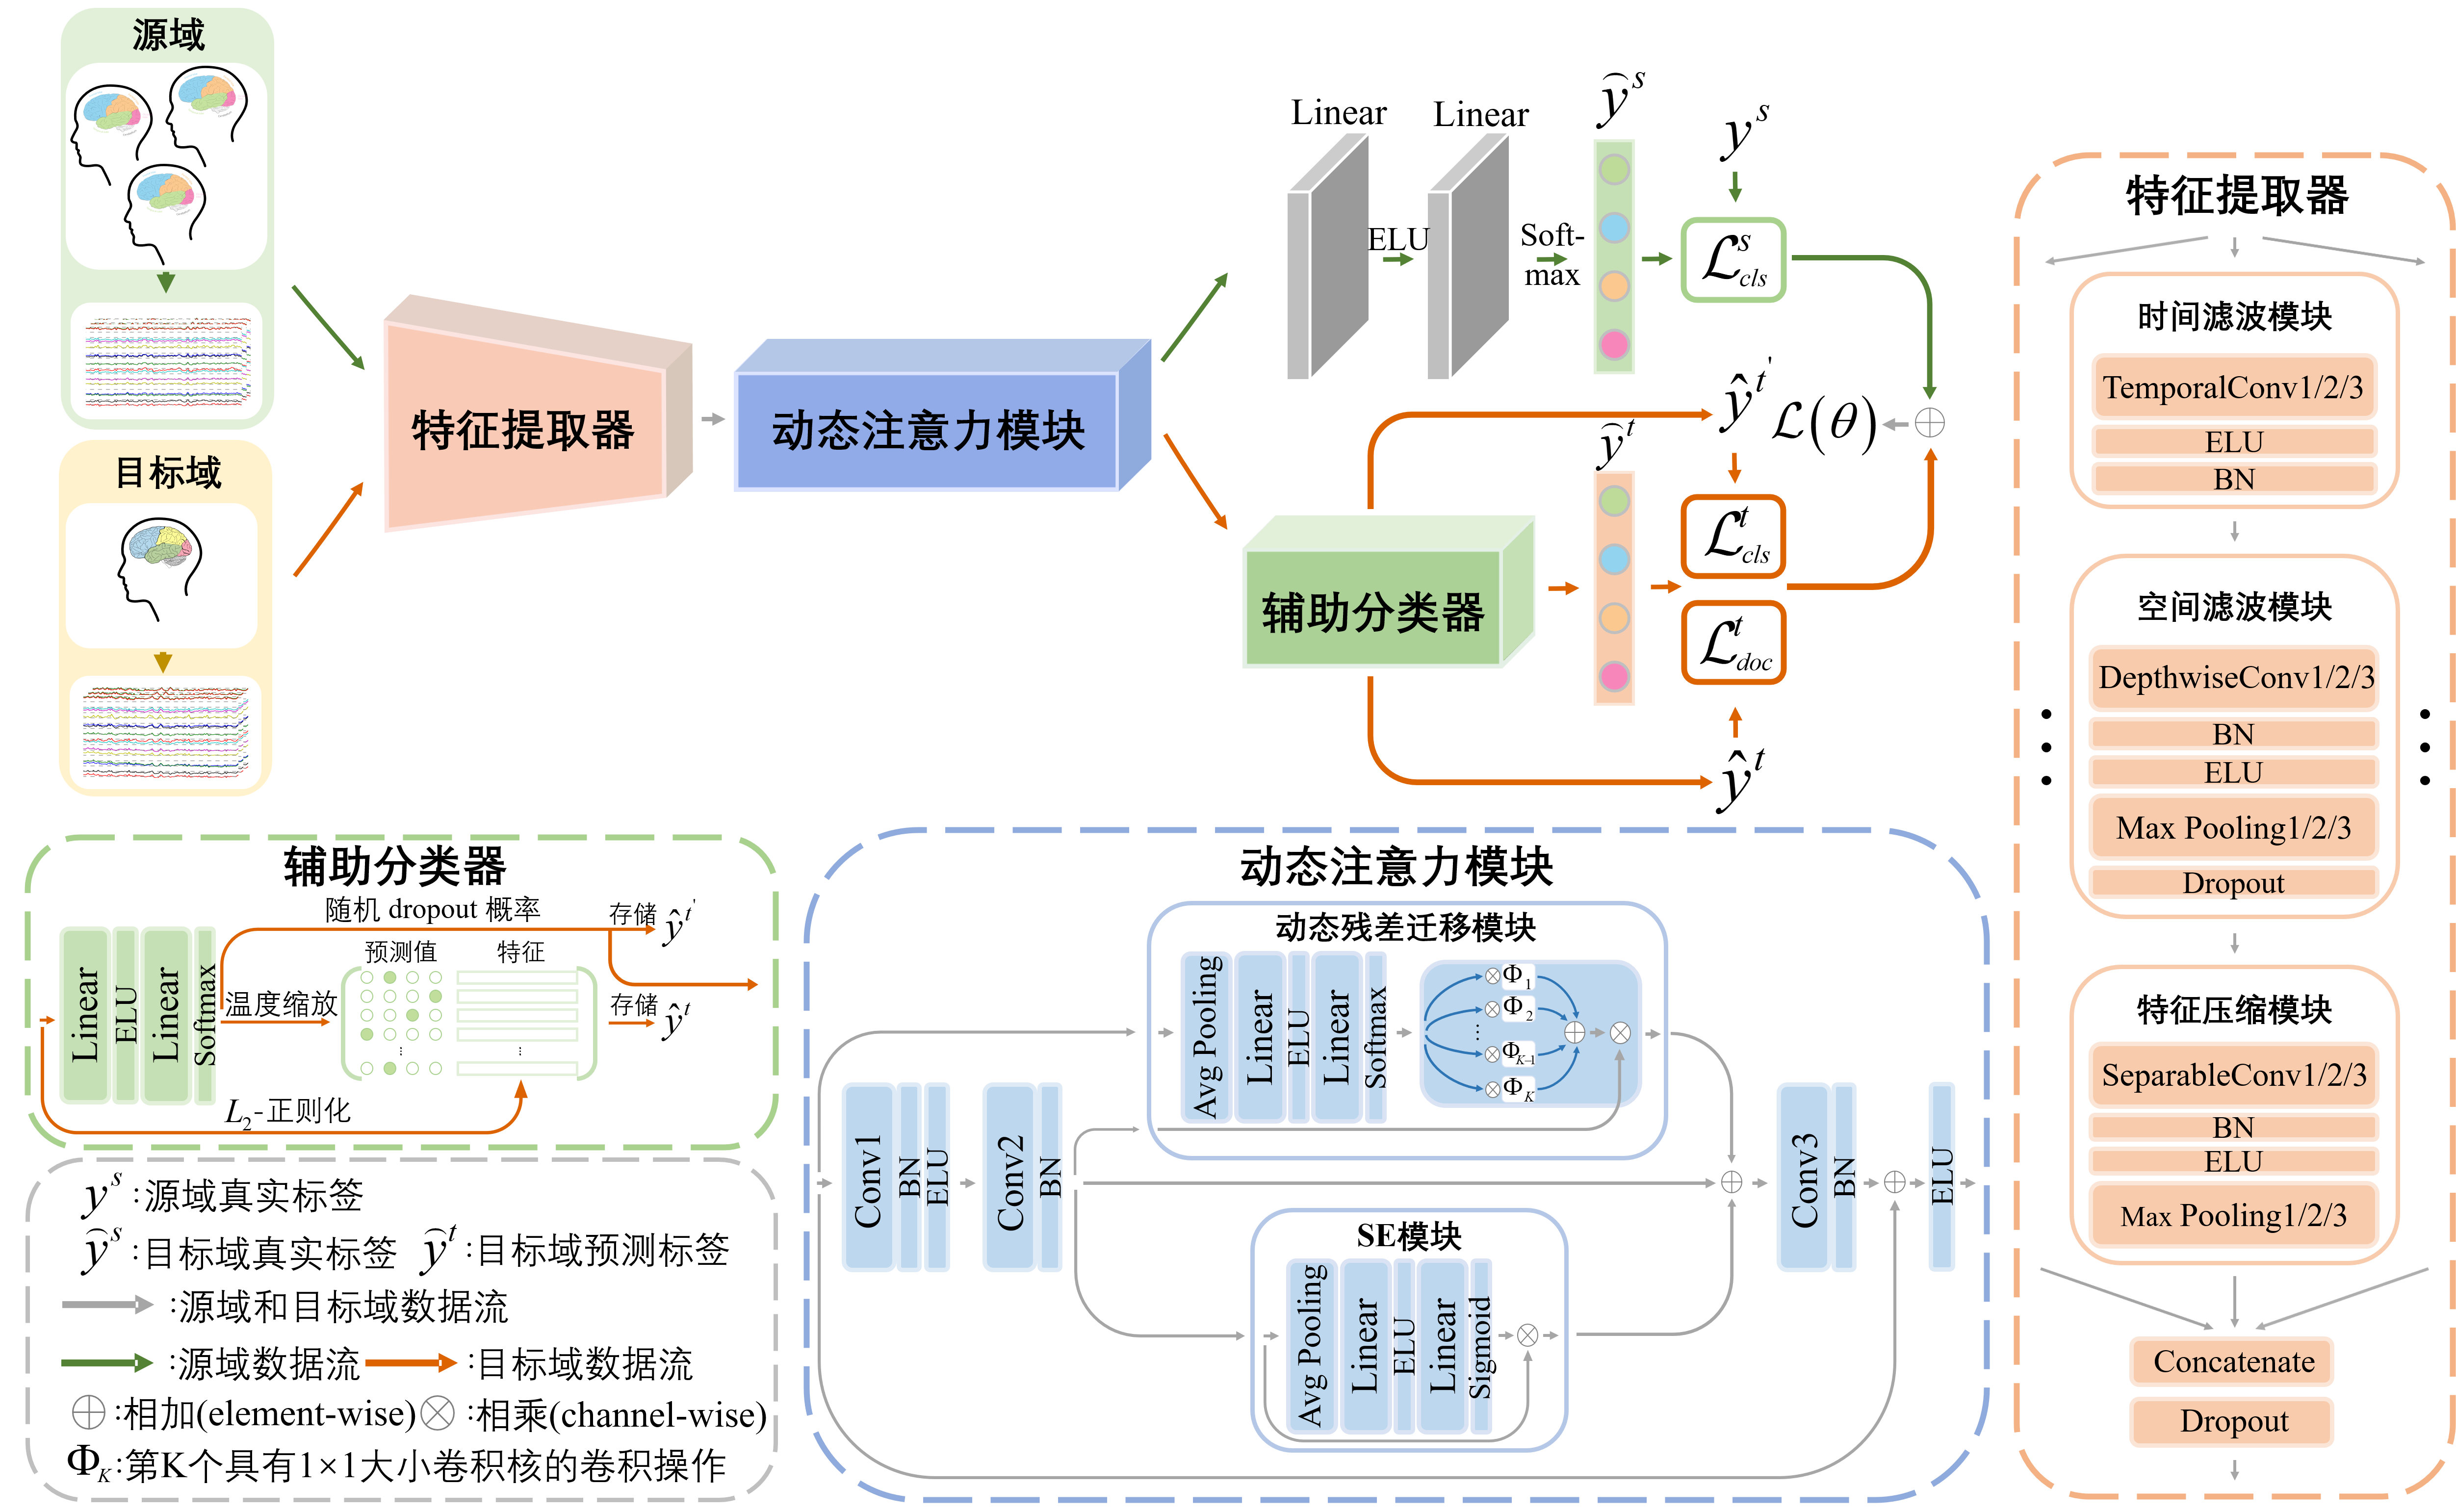
\includegraphics[width=1\textwidth]{主模型图_v1.png}
\caption{迭代自训练多被试域适模型示意图}
\label{fig_4_1}
\end{figure*}

\subsection{问题定义}
本章利用域适应算法实现MI-BCI系统的跨被试同时跨时段分类辨识,为了问题描述的准确性,在这里进行详细的问题定义。

(1) 定义和符号

设$D_{s_{j}}=\left\{\left(x_{i}^{s_{j}}, y_{i}^{s_{j}}\right)\right\}_{i=1}^{n^{s_{j}}}, j \in\{1, \ldots, N\}$代表拥有${n^{s_{j}}}$个有标签样本的$N$个源域中的第$j$个域。其中的第$i$个样本$x_{i}^{s_{j}} \in \mathbb{R}^{C \times L}$拥有$C$个通道和$L$个样本点,${y_{i}^{s_{j}}}$为第$i$个样本所对应的真实标签。${n^{s_{j}}}$代表源域$S_{j}$中所包含的EEG样本数。相似的,将包含${n^{t}}$个未标记样本的目标域$\mathcal{T}$定义为$D_{t}=\left\{\left(x_{i}^{t}\right)\right\}_{i=1}^{n^{t}}$。所有域中的样本均包含$N_{c}$个不同的类别。

考虑到不同域之间的分布差异$P_{S}\left(D_{s}\right) \neq P_{\mathcal{T}}\left(D_{t}\right)$,从不同域提取到的数据联合分布$P$需要进行对齐。假设存在一个由参数$\theta$组成的模型$M_{\theta}$,其能够减少不同域分布之间的差异,并正确地将目标域样本$x_{i}^{t}$映射到相应的类别,那么这一模型便能够解决本章所针对的问题。因此,本章所涉及的分类任务的最终目的,就是找到一个满足这一要求的模型。

(2) 基于MI-BCI系统的多被试迁移任务

本章节所进行的所有实验均满足本节中所设定的迁移学习场景,具体内容如下:选取MI数据集中某一特定被试的EEG信号作为目标域$\mathcal{T}$,其余的其他被试作为源域$\mathcal{S}=\left\{\mathcal{S}_{1}, \ldots, \mathcal{S}_{N}\right\}$,二者共同对分类器完成校准。为了进一步提高模型的实用性,设定源域数据无法携带它们的域标签,这意味着来自不同被试的数据将被随机混合并作为一个统一的源域使用。遵循Choi给出的定义\cite{4-1},本文的应用场景被定义为多被试迁移(Multi-subject Transfer)任务。

\subsection{模型结构}
本章节将从ISMDA的三大组成部分:多通道时空滤波特征提取器(MTSF),动态注意力模块(DAM)以及基于面向域分类器的迭代自训练(DCIS)分别展开介绍。

(1) 多通道时空滤波特征提取器

鉴别性特征的提取有助于提高模型下游的EEG信号辨识准确性,并且决定了模型的性能基线。本文受到EEGNet\cite{4-2}——一个成功的、可推广的EEG分类模型的启发,提出了MTSF模块。MTSF模块由三个分支组成,每个分支针对EEG信号的特点分为三个级联模块,即时间滤波模块、空间滤波模块和特征压缩模块。

\begin{table}[h]
	\caption{多通道时空滤波模块的结构参数 \label{tab4-1}}
	\centering
	\wuhao{
        \setlength{\tabcolsep}{2mm}{
		\begin{tabular}{cccc}
		  \toprule
            \textbf{模块}                      & \textbf{网络层} &\textbf{参数} & \textbf{输出} \\
            \midrule
            \textbf{输入}                       & -      &  -  & $(1, \mathrm{C}, \mathrm{L})$\\
            \midrule
            \multirow{3}*{时间滤波模块}  & TemporalConv1/2/3 & $1\times18$ / $1\times24$ / $1\times36$ $@$$F_{1}$ & $(F_{1}, C, L)$\\
                                       & $ELU$                      & & $(F_{1}, C, L)$\\ 
                                       & $BN$      & & $(F_{1}, C, L)$\\ 
            \midrule
            \multirow{5}*{空间滤波模块}  & DepthwiseConv1/2/3 & $C \times 1$$@$$F_{1}*D$, padding=`VALID'& $(F_{1}*D, 1, L)$\\
             & $BN$      &  & $(F_{1}*D, 1, L)$   \\ 
             & $ELU$                      &  & $(F_{1}*D, 1, L)$       \\ 
             & Max Pooling1/2/3         & stride=$(1, 8)$  & $(F_{1}*D, 1, L//8)$ \\ 
             & Dropout                  &  & $(F_{1}*D, 1, L//8)$          \\
            \midrule
            \multirow{6}*{特征压缩模块}   & SeparableConv1/2/3 & $1 \times 16$$@$$F_{2}$& $(F_{2}, 1, L//8)$\\
             & $BN$      & & $(F_{2}, 1, L//8)$\\ 
             & $ELU$                     & & $(F_{2}, 1, L//8)$    \\ 
             & Max Pooling1/2/3         & stride=$(1, 8)$ & $(F_{2}, 1, L//64)$   \\ 
             & Concatenate              &   & $(F_{2}*3, 1, L//64)$          \\ 
             & Dropout                  &   & $(F_{2}*3, 1, L//64)$          \\ 
             \bottomrule
    
       \end{tabular}
       }}
\end{table}


1) 时间滤波模块:在时间滤波模块中,特征提取器的三个分支首先对EEG信号进行时间卷积(Temporal Convolution)。具体来说,特征提取器的三个分支可以被看作是具有不同参数的时间滤波器,其卷积核大小分别为(1,36)、(1,24)与(1,18),滤波器数量为$F_1$。这三个分支首先采用指数线性单元(Exponential Linear Unit,$ELU$)来激活经过时间滤波的EEG特征图,以使模型获得足够的非线性表征能力。在$ELU$之后,对特征图进行批归一化操作(Batch Normalization, $BN$)。

2) 空间滤波模块:在空间滤波模块中,首先利用大小为($C$,1)的深度卷积(Depth-wise Convolution)对时间滤波模块输出的特征图进行空间滤波。对时间滤波模块输出的每个特征图,深度卷积均训练$D$个滤波器,这意味着每个深度卷积都由$F_1*D$个滤波器组成。其次,采用批归一化操作和$ELU$激活函数对空间特征图进行进一步处理。紧接着,应用大小为(1,8)的最大池化层(Max Pooling)以扩展模型的感受野。最后,引入概率为0.5的Dropout层以提高数据表示的稀疏性,减少冗余。

3) 特征压缩模块:为了在有限的计算资源中提取更加抽象化的特征,特征压缩模块采用了可分离卷积(Separable Convolution)来处理空间滤波器的输出。可分离卷积的卷积核大小和滤波器数量分别为(1,16)和$F_2$($F_2$的大小被设定为$F_1*D$)。之后,为了减少特征图的维度,引入大小为(1,8)的最大池化层。在本文中,$F_{1}$被设定为8,$D$被设定为2,$C$由数据集决定。

三个分支的输出特征将被串联(Concatenate)并扩展成一个一维向量,它以0.5的概率通过Dropout层传递给动态注意力模块。MTSF的具体参数和输出维度见表\ref{tab4-1}。

(2) 动态注意力模块

模型$M_{\theta}$被称为静态或动态,取决于其参数$\theta$是否随输入样本$x$而变化,即$\theta=\theta(x)$并且$x\in S \bigcup \mathcal{T}$。当$M_{\theta}$为动态模型时,其可以根据不同输入的特点动态地调整参数$\theta$。此时$\theta$不再需要关联于域,而是直接关联于样本。更进一步,由于模型能够直接根据样本特点实现参数调整,此时源域便不再需要与目标域进行对齐,即不同域之间不再具有固定的边界。此外,由于不再有对域信息的依赖,此时的训练过程不需要区分不同的源域,也不再需要引入域标签,这有效地降低了训练的复杂度。综上所述,在下文的描述中,源域均使用$S$来表示。

受Li等人\cite{4-3}所提出的动态残差迁移模型的启发,DAM被引入ISMDA中。此外,根据Li等人\cite{4-3}的研究,动态迁移模型可以简单地通过聚合静态矩阵和残差模块来实现,因此本章所设计的DAM模型由静态模块和动态残差模块两部分组成:
\begin{equation}
\label{deqn_ex1}
W(x)=W_{0}+\Delta {W}({x}),
\end{equation}
其中$W_{0}$代表由静态卷积矩阵组成的静态模块,$\Delta {W}({x})$代表由动态残差矩阵组成的动态残差模块。动态残差矩阵由一组通道注意力模块和子空间路由模块构成:
\begin{equation}
\label{deqn_ex2}
\Delta {W}({x})={\Lambda}({x}) {W}_{0}+\sum_{i=1}^{K} \pi_{i}(x){\Phi}_{i}.
\end{equation}

${\Lambda}({x}) {W}_{0}$代表了通道注意力模块,而${\Lambda}({x})$是一个大小为$C_{\text {out }} \times C_{\text {out }}$的对角矩阵,其中$C_{\text {out }}$代表了输出特征图的通道数量。在本章中,通道注意力模块由Squeeze-and-Excitation模块实现\cite{4-4}。

子空间路由模块$\sum_{i=1}^{K} \pi_{i}(x){\Phi}_{i}$是$K$($K=4$)个静态矩阵${\Phi}_{i}$的线性组合,其权重由输入$x$所决定。模型权重空间中的投影由动态参数$\pi_{i}(x)$和静态矩阵${\Phi}_{i}$的乘积来选择,这本质上是选择不同的子空间来路由不同的输入$x$。动态参数由一个平均池化(Average Pooling)层和两个全连接(Linear)层组成的注意力分支所产生。在本文中,采用$softmax$对${\Phi}_{i}$进行归一化。

如图\ref{fig_4_1}所示,受ResNet中瓶颈结构的启发,特征提取器输出的特征通道数首先通过一组相继连接的卷积层、批归一化层和$ELU$激活函数转换为48,然后进入DAM。在通道注意力模块和子空间路由模块之后,特征向量将被拼接,特征向量的通道数通过一组卷积层和批量归一化层被扩展到原先的四倍。最后,经由残差连接,DAM的输出传递给下一模块。

(3) 基于面向域分类器的迭代自训练

为了削弱分布偏移所带来的影响,避免模型过于偏向源域数据,本节引入了一种新的伪标签训练策略——DCIS。DCIS包含ATDOC和PACC两种伪标签算法,以迭代自训练的方式分两个阶段分别引入模型的训练过程中。两个阶段均采用了相同数量的epochs以保证模型的最终性能。

1) 面向域分类器:考虑到基于邻域聚合的ATDOC模型显著优于已有的域对齐技术和半监督学习算法\cite{4-5},本节采用其作为DCIS中的第一种伪标签生成策略。鉴于目标域的标签稀疏性,one-hot伪标签由下式得到\cite{4-6}:
\begin{equation}
\label{deqn_ex3}
\hat{y}^{t}=\arg \max _{k} p_{k}^{t},
\end{equation}
其中$p^{t}$是输入$x^{t}$的预测结果,为$N_{C}$维向量。利用MTSF和DAM提取的特征,经由一组全连接层组成的分类器即可获得$p^{t}$。

在本文中,为了防止预测中可能出现的混淆问题,首先利用$a=0.5$的温度缩放(Temperature Scaling)\cite{4-7}对预测结果$p^{t}$进行锐化:
\begin{equation}
\label{deqn_ex4}
{\check{p}_{k}^{t}}=(p_{k}^{t})_{{}}^{\frac{1}{a}}/\sum\nolimits_{k=1}^{{{N}_{c}}}{(p_{k}^{t})_{{}}^{\frac{1}{a}}}.
\end{equation}
从上式可以看出,随着$a$逐渐收敛为零,预测值$p^{t}$将从概率分布坍缩到一个特定的点,即某一具体类别。之后,当前目标域样本的锐化预测值${\check{p}_{k}^{t}}$将与它对应的$L_{2}$正则化特征向量
\begin{equation}
\label{deqn_ex5}
f^{t'}=f^{t} /\left\|f^{t}\right\|_{2}
\end{equation}
根据其在数据集中的索引位置,一起被存储在一个独立的模块中,即记忆库(Memory Bank)。其中$f^{t}$是由DAM输出得到的特征向量。在每一批目标域样本通过模型后,新的样本将被添加到记忆库中。

按照邻域聚合策略,利用余弦相似度检索出与每个样本特征向量最接近的$m$($m=5$)个其他样本。然后,通过对最接近的$m$个样本的预测值进行平均,得到当前样本的伪标签:
\begin{equation}
\label{deqn_ex6}
{\hat{q}_{k}^{t}}=\frac{1}{m}\sum\nolimits_{j\in {{\mathcal{N}}_{i}}}\check{p}_{j,k}^{t},
\end{equation}
其中${\mathcal{N}}_{i}$代表了记忆库中所有样本所携带的索引集。在完成所有样本的迭代后,记忆库将建立一个反映目标域全局结构的分类器,而无需学习任何新的参数。

由面向域分类器得到的目标域样本的伪标签为:
\begin{equation}
\label{deqn_ex7}
\hat{y}^{t}=\arg \max _{k} \hat{q}_{k}^{t}.
\end{equation}

然而,位于密度较高邻域的样本具有较高的正确分类概率,这可以直接反映在${\hat{q}}^{t}$中最大子项的数值大小上。因此,采用${\hat{q}}^{t}$作为伪标签的置信度权重,得到目标域样本的面向域分类器交叉熵损失:
\begin{equation}
\label{deqn_ex8}
\min{\mathcal{L}_{doc}^{t}=-\mathbb{E}_{x^{t}\sim P_\mathcal{T}}\sum\nolimits_{k=1}^{N_c}{\mathbbm{1}_{\left[{\hat{y}}^{t}=k\right]}{\hat{q}}_k^{t} \log {p_k^{t}}}}.
\end{equation}

2) 迭代自训练:在ATDOC之外,DCIS还建立了一个由两个顺序连接的全连接层组成的分类器。由MTSF和DAM输出的特征将首先被扩展成为一维向量,并传递给具有500个单元的第一个全连接层,如图\ref{fig_4_1}所示。这个全连接层采用$ELU$作为激活函数。接下来,拥有$N_C$个单元的第二个全连接层采用$softmax$激活函数来获得最终的分类结果。

根据常见的自训练策略,所有的目标域样本都必须事先进行伪标签化。然而在一定程度的训练之前,网络无法对目标域的样本进行正确的分类。综上所述,本文引入了迭代式自训练策略。在迭代式自训练的第一阶段,首先使用ATDOC生成伪标签来训练网络。在第二阶段,ATDOC将被冻结,从第一阶段得到的经过完善训练的模型所产生的新伪标签$\hat{y}^{t^{'}}$,将被用来对当前模型进行进一步微调。在这一时刻,虽然模型具有足够的分类精度,但其不一定经过足够的校准,即模型的$softmax$输出可能并不是决策置信度的真实反映\cite{4-7}。具体来说,此时的伪标签中混入了大量高置信度的错误分类结果,此时将这种充满噪声的标签引入未经校准的模型毫无疑问是灾难性的。考虑到置信度和确定性问题,迭代式自训练的第二阶段的伪标签是:
\begin{equation}
\label{deqn_ex9_addation1}
\hat{p}_{k}^{t^{'}} = \left\{\begin{array}{cl}
\overline{p}_{k}^{t},&\text{if}\ {u}({p}_{k}^{t,i}) \leq {k}_{u}\ \text{and}\ \ \overline{p}_{k}^{t} \geq {k}_{c}\\ 
discard,&{\text{otherwise}}
\end{array}\right.,
\end{equation}
其中$i=1,2,\cdots,U$。在第一阶段得到的模型基础上,随机设置其Dropout概率$U$次,并对同一样本进行$U$次预测以获得一组${p}_{k}^{t,i}$。$\overline{p}_{k}^{t}$代表了$U$个${p}_{k}^{t,i}$的平均值。$\overline{p}_{k}^t$可以被看做是伪标签置信度的评价指标,这源于一个事实,即每个具有不同Dropout概率的模型可以被视为具有不同参数的子模型,众多子模型的联合投票结果将会更为鲁棒与可信。同时,受预期校准误差(Expected Calibration Error)\cite{4-7}和模型不确定性(Model Uncertainty)之间的相关性启发\cite{4-9},同一样本在不同预测值${u}({p}_{k}^{t})$上的置信度方差被视为不确定性的评价指标。最终,满足置信度与不确定性指标的$\overline{p}_{k}^t$,即方差低于阈值${k}_{u}$而均值高于阈值${k}_{c}$的伪标签,将会在第二阶段得以保留。不符合要求的标签将被直接舍弃。
\begin{equation}
\label{deqn_ex9_addation2}
\hat{y}^{t^{'}} = \arg \max _{k} (\hat{p}_{k}^{t^{'}}).
\end{equation}

此外,鉴于容易区分的类别会有更多的样本符合阈值条件,因此本章节引入了一个样本平衡策略,以避免模型在训练过程中产生对于某类样本的偏向性。具体来说,通过计算所有符合条件的样本并依次保留具有高置信度和低不确定性者,使每个类别的样本数量保持一致。在第二阶段,伪标签经过每100个epoch将被更新一次,以保证伪标签的可靠性随着训练进程而逐步提高。第二阶段的自训练交叉熵损失如下:
\begin{equation}
\label{deqn_ex9}
\min{\mathcal{L}_{cls}^t=-\mathbb{E}_{x^t\sim P_\mathcal{T}}\sum\nolimits_{k=1}^{N_c}{\mathbbm{1}_{\left[{\hat{y}}^{t^{'}}=k\right]} {\log {p_k^t}}}}. 
\end{equation}

为了避免可能出现的不确定性,在本章节中,设定$U$为30,设定${k}_{u}$为0.05,设定${k}_{c}$为0.7。

\begin{algorithm}[!h]
\algsetup{linenosize=\small}
\small
\setcounter{algorithm}{0}
\floatname{algorithm}{\small{算法4 -}} 
\caption{\small{ISMDA的算法流程.}}\label{alg:alg1}
\begin{algorithmic}
\STATE 
\STATE{\textbf{输入:}}\ 源域的EEG时间序列以及对应标签: $ D_{s}=\left\{\left(x_{i}^{s}, y_{i}^{s}\right)\right\}_{i=1}^{n^{s}}$;
\vspace{0.22cm}
\STATE \hspace{0.90cm}\ 目标域的EEG时间序列: $ D_{t}=\left\{\left(x_{i}^{t}\right)\right\}_{i=1}^{n^{t}}$;
\vspace{0.22cm}
\STATE \hspace{0.90cm}\ DCIS中的近邻样本数: $m$;
\vspace{0.22cm}
\STATE \hspace{0.90cm}\ 模型$M$的学习率: $\eta$;
\vspace{0.22cm}
\STATE \hspace{0.90cm}\ 源域与目标域数据的batch size: $n$;
\vspace{0.22cm}
\STATE \hspace{0.90cm}\ 单个训练阶段的epoch数:  $E$.
\vspace{0.22cm}
\STATE{\textbf{输出:}}\ 训练后的模型参数: $\Theta$.
\vspace{0.22cm}
\STATE{\textbf{初始化:}}\ 初始模型参数:  $\Theta$;
\vspace{0.22cm}
\STATE \hspace{1.3cm}\ 计算公式(\ref{eq:12B})中权重$\lambda$的初始值: $\frac{1}{n^{s} \times E}$;
\vspace{0.22cm}
\STATE \hspace{1.3cm}\ 记忆库初始化. 
\vspace{0.22cm}
\STATE 1. \textbf{For} \textbf{训练阶段}$\in[1,2]$ \textbf{do}:
\vspace{0.22cm}
\STATE 2. \hspace{0.4cm}根据公式(\ref{eq:12})更新调节参数 $\alpha(T), \beta(T), \gamma(T)$;
\vspace{0.22cm}
\STATE 3. \hspace{0.4cm}\textbf{For} $T \in[1, E]$ \textbf{do}:
\vspace{0.22cm}
\STATE 4. \hspace{0.8cm}当\textbf{训练阶段}等于2并且\textbf{$T$}被100整除时,利用公式(\ref{deqn_ex9_addation1})生成目标域伪
\vspace{0.22cm}
\STATE \hspace{1.16cm} 标签:$M$: $\left\{\hat{y}_{i}^{t}\right\}_{i=1}^{n_{t}} \leftarrow \Theta, D_{t}^{\prime}=D_{t} \cup\left\{\hat{y}_{i}^{t}\right\}_{i=1}^{n_{t}}$;
\vspace{0.22cm}
\STATE 5. \hspace{0.8cm}从源域$D_{S}$中取出一个batch的源域样本$\left\{\left(x_{i}^{s},y_{i}^{s}\right)\right\}_{i=1}^{n}$;
\vspace{0.22cm}
\STATE 6. \hspace{0.8cm}从目标域$D_{t}^{\prime}$中取出一个batch的目标域样本$\left\{\left(x_{i}^{t},\hat{y}_{i}^{t}\right)\right\}_{i=1}^{n}$;
\vspace{0.22cm}
\STATE 7. \hspace{0.8cm}\textbf{For} \textbf{样本} $\in$ batch \textbf{do}:
\vspace{0.22cm}
\STATE 8. \hspace{1.2cm}更新公式(\ref{eq:12B})中的权重$\lambda$;
\vspace{0.22cm}
\STATE 9. \hspace{1.2cm}利用公式(\ref{deqn_ex10})计算源域有监督损失$\mathcal{L}_{cls}^{s}$;
\vspace{0.22cm}
\STATE 10.\hspace{1.15cm}计算邻域聚合伪标签$\hat{q}^{t}$;
\vspace{0.22cm}
\STATE 11.\hspace{1.15cm}根据公式(\ref{deqn_ex8})和公式(\ref{deqn_ex9})计算目标域无监督损失$\mathcal{L}_{d o c}^{t}$和$\mathcal{L}_{c l s}^{t}$;
\vspace{0.22cm}
\STATE 12.\hspace{1.15cm}根据公式(\ref{deqn_ex11})计算整体损失$\mathcal{L}(\theta)$;
\vspace{0.22cm}
\STATE 13.\hspace{1.15cm}优化模型参数: $\Theta \leftarrow \Theta-\mu \frac{\partial \mathcal{L}}{\partial \Theta}$;
\vspace{0.22cm}
\STATE 14.\hspace{1.15cm}更新记忆库;
\vspace{0.22cm}
\STATE 15. {\textbf{结束}};
\vspace{0.22cm}
\STATE 16. 返回训练好的模型参数$\Theta$;
\end{algorithmic}
\end{algorithm}

(4) 网络优化框架

由MTSF、DAM和DCIS组成的ISMDA框架,利用基于源域数据的有监督学习和基于目标域数据的自训练策略在两个迭代的训练阶段进行逐步优化。ISMDA的整个训练流程详见算法4 -\ref{alg:alg1}。具体来说,$M_\theta$的参数可以通过同时最小化源域中的有监督学习损失和目标域中的自训练损失来完成优化。考虑到源域和目标域之间数据量的差异性,采用带有标签平滑正则化(Label-Smoothing Regularization)\cite{4-8}的交叉熵损失作为源域的损失函数:
\begin{equation}
\label{deqn_ex10}
\min\mathcal{L}_{cls}^{s}=-\mathbb{E}_{\left(x^{s}, y^{s}\right) \sim P_{s}} \sum\nolimits_{k=1}^{N_{c}} q_{k}^{\prime} \log {p_k^s},
\end{equation}
其中$p_k^s$是源域样本$x^{s}$的预测值的第$k$维,$q^{\prime}$是经过标签平滑后的one-hot真实标签。基于上述描述,ISMDA的整体损失函数可以表征为:
\begin{equation}
\label{deqn_ex11}
\mathcal{L}(\theta)=\alpha(T) \mathcal{L}_{c l s}^{s}+\beta(T) \mathcal{L}_{d o c}^{t}+\gamma(T)\mathcal{L}_{cls}^{t}
\end{equation}
其中$\alpha(T)$,$\beta(T)$,$\gamma(T)$是被用来在训练进程$T$中平衡有监督学习和自训练的调节参数。为了获得模型的最佳性能,在不同的训练阶段采用了不同的参数值:
\vspace{-2mm}
\begin{subequations}
\label{eq:12}
\begin{align}
\alpha(T) =& \left\{\begin{array}{rll}
\alpha_{0},&T\leq E&\\
0.1\times\alpha_{0},&E<T\leq 2E,&
\end{array}\right.\label{eq:12A}\\[1.5mm] 
\beta(T) =& \left\{\begin{array}{rll}
\ \ \lambda \times \beta_{0} ,&T \leq E&\\
0 ,&E<T \leq 2E,&
\end{array}\right.\label{eq:12B}\\[1.5mm]
\gamma(T) =& \left\{\begin{array}{rll}
\ \ \ \ \ \ \ \ \ 0 ,&T\leq E& \\
\gamma_{0} ,&E<T \leq 2E,&
\end{array}\right.\label{eq:12C}
\end{align}
\end{subequations}
考虑到记忆库在训练的第一阶段开始时,仅仅只能获取较为粗略的原始特征向量,权重$\lambda$采用了线性缩放策略(Linearly Scheduling Skill)以保证ATDOC在初始时不会对模型产生较大影响。而随着记忆库中鉴别性表征的增加,$\lambda$以$\frac{1}{n^{t} \times E}$为步长,逐渐从$\frac{1}{n^{t} \times E}$增长到1。$E$代表了一个训练阶段所需要进行的epoch数。$\alpha_{0}$,$\beta_{0}$,$\gamma_{0}$在BCI IV IIa Dataset和JS-MI Dataset上被设定为1,0.2,2,而在High Gamma Dataset和Additional Dataset上$\alpha_{0}$,$\beta_{0}$,$\gamma_{0}$被设定为1,0.02,2。 值得注意的是,$\mathcal{L}_{c l s}^{s}$的权重$\alpha_{0}$在第二个训练阶段被乘以了一个缩放系数,其大小为0.1。




\section{实验描述}
本章详细介绍了对比试验所引入的四种数据集和八种对比方法,并描述了对比实验的具体流程与参数设计。

\subsection{运动想象数据集}
为了评估本章所提出的基于多被试动态迁移与迭代自训练的EEG辨识算法的有效性,并进一步考量JS-AINS-40设备的实际使用效果。本章引入了三个公开的MI-EEG数据集与一个JS-AINS-40采集的MI-EEG数据集来评估模型的性能。公开数据集包括第四次BCI竞赛中的IIa数据集(BCI IV IIa Dataset)\cite{4-10}、High Gamma Dataset (HGD)\cite{4-11}以及Kwon等人采集的数据集(Additional Dataset)\cite{4-12}。JS-AINS-40采集的MI-EEG数据集称为JS-MI Dataset。所有的数据集都捕捉到了人脑的电生理活动,这些活动在特定的频段上与外部刺激的反应相吻合。

(1) 数据集I:BCI IV IIa Dataset

BCI IV IIa Dataset以250 Hz的采样率在两个时段中利用22个EEG电极和3个眼电电极记录了9名不同受试者的MI信号。此外,其包含的两个时段是在不同日期采集的。在实验开始前,每个受试者都被告知将会进行四种类型的MI任务,包括左手、右手、脚和舌头。每个时段均包括288个4秒钟的MI实验。采集结束后,数据集作者使用0.5 Hz到100 Hz的带通滤波器与50 Hz的工频陷波滤波器对原始EEG信号进行了预处理。本章所使用的数据只包括22个EEG通道,直接舍弃了3个眼电通道。

(2) 数据集II:High Gamma Dataset

与其他MI数据集相比,High Gamma Dataset在采集过程中引入了高分辨率的放大器、电磁屏蔽和全光学去耦,获得了高质量的EEG信号。High Gamma Dataset采集了14名健康受试者的四个MI类别EEG,包括左手、右手、双脚和休息(没有运动,但与其他类别具有相同的视觉引导)。每名受试者都经由128通道电极在500 Hz采样率下采集了1040次MI实验数据。根据Schirrmeister等人\cite{4-11}的工作,在本章中High Gamma Dataset数据集被降采样为250 Hz,并且只保留其中的44个电极以去除冗余信息。

(3) 数据集III:Additional Dataset

Additional Dataset是一个二分类MI数据集,包含54名健康的受试者。在所有受试者中,38人是初次参与EEG实验,其他人则拥有EEG实验经历。每名受试者均被要求在指导下进行四个时段的左/右手MI,共400次实验,每次持续4秒。Additional Dataset使用62个EEG电极在1000 Hz采样率下完成了EEG信号采集。遵循Zhang等人\cite{4-13}的工作,数据集被降采样至250 Hz。

(4) 数据集IV:JS-MI Dataset

为验证JS-AINS-40的实际使用效果,设计全新的MI实验以对其性能进行评估。在本次实验中获得的数据集即JS-MI Dataset,实验的详细内容如下所述。

本次实验共选取了9名年龄在20-30岁之间的受试者(5名男性,4名女性),这些受试者均身体健康,无视力及大脑相关疾病,没有吸毒史,且在近几周保持了健康的作息。9名受试者中有5人曾参与EEG实验,4人不具备相关的实验经历。本实验经过了天津医科大学总医院的伦理委员会的审查,并签署了知情同意书。

为了验证的合理性,实验的整体流程在BCI IV IIa Dataset的基础上进行设计。首先,每名受试者在不同日期完成两次EEG数据采集(两个时段),每次实验均保持相同的流程。其次,实验包括四个基本类别的运动想象任务,分别为左手、右手、双脚以及舌头。四个类别在两个时段中以随机的顺序出现,每个类别均出现144次,即每名被试在两个时段中一共采集576段EEG数据。
在实验开始前,对所有受试者进行了实验内容的相关介绍,并让所有受试者保持舒适的坐姿佩戴EEG电极帽目视电脑屏幕中心,与电脑屏幕保持约70 cm的距离。在确认受试者准备就绪后,运行JS-AINS-40系统进行数据采集。

\begin{figure}[h]
	\centering
	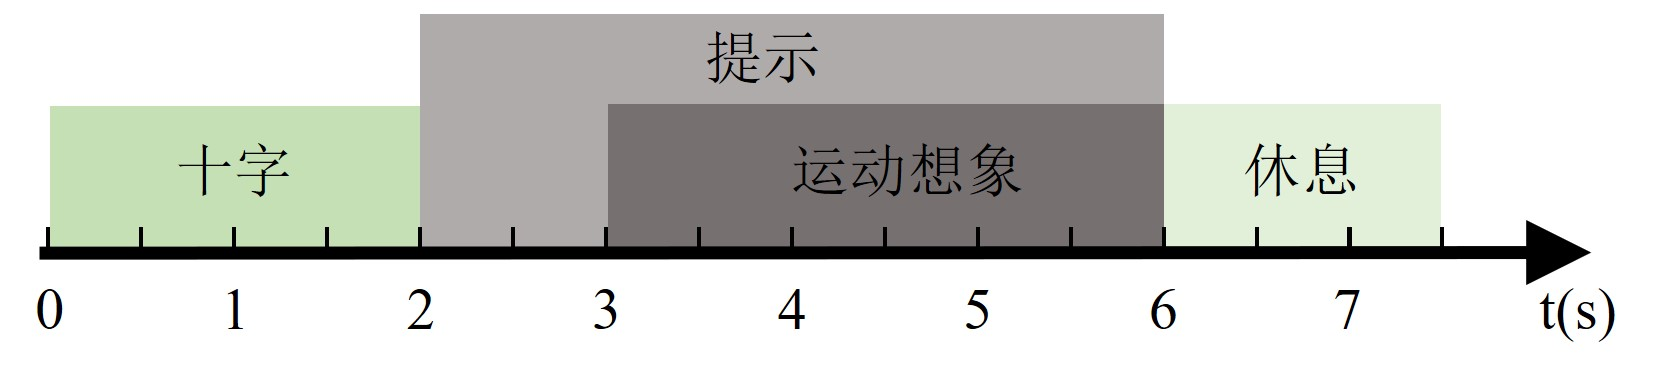
\includegraphics[width=0.5\textheight]{figures/运动想象实验流程.jpg}
	\caption{JS-MI Dataset的实验流程} 
	\label{fig_4_2}
\end{figure}

实验中,遵循图\ref{fig_4_2}完成实验流程。每次实验开始时($t=0$ s),屏幕中心会出现固定的十字以提醒受试者保持专注。在两秒后($t=2$ s),屏幕中心会出现与MI类别相对应的照片,提示受试者完成相应的想象任务,如图\ref{fig_4_3}。照片提示将会一致维持,直至本次实验结束($t=6$ s)。在照片开始显示的1秒后($t=3$ s),系统左上角将提示受试者当前应进入想象阶段,右上角则给出了当前任务的剩余时间。当想象结束后($t=6$ s),受试者将会得到1.5秒的休息。在整个实验过程中,始终开启50 Hz工频陷波滤波器对数据进行滤波。

\vspace{7mm}

\begin{figure}[h]
	\centering
	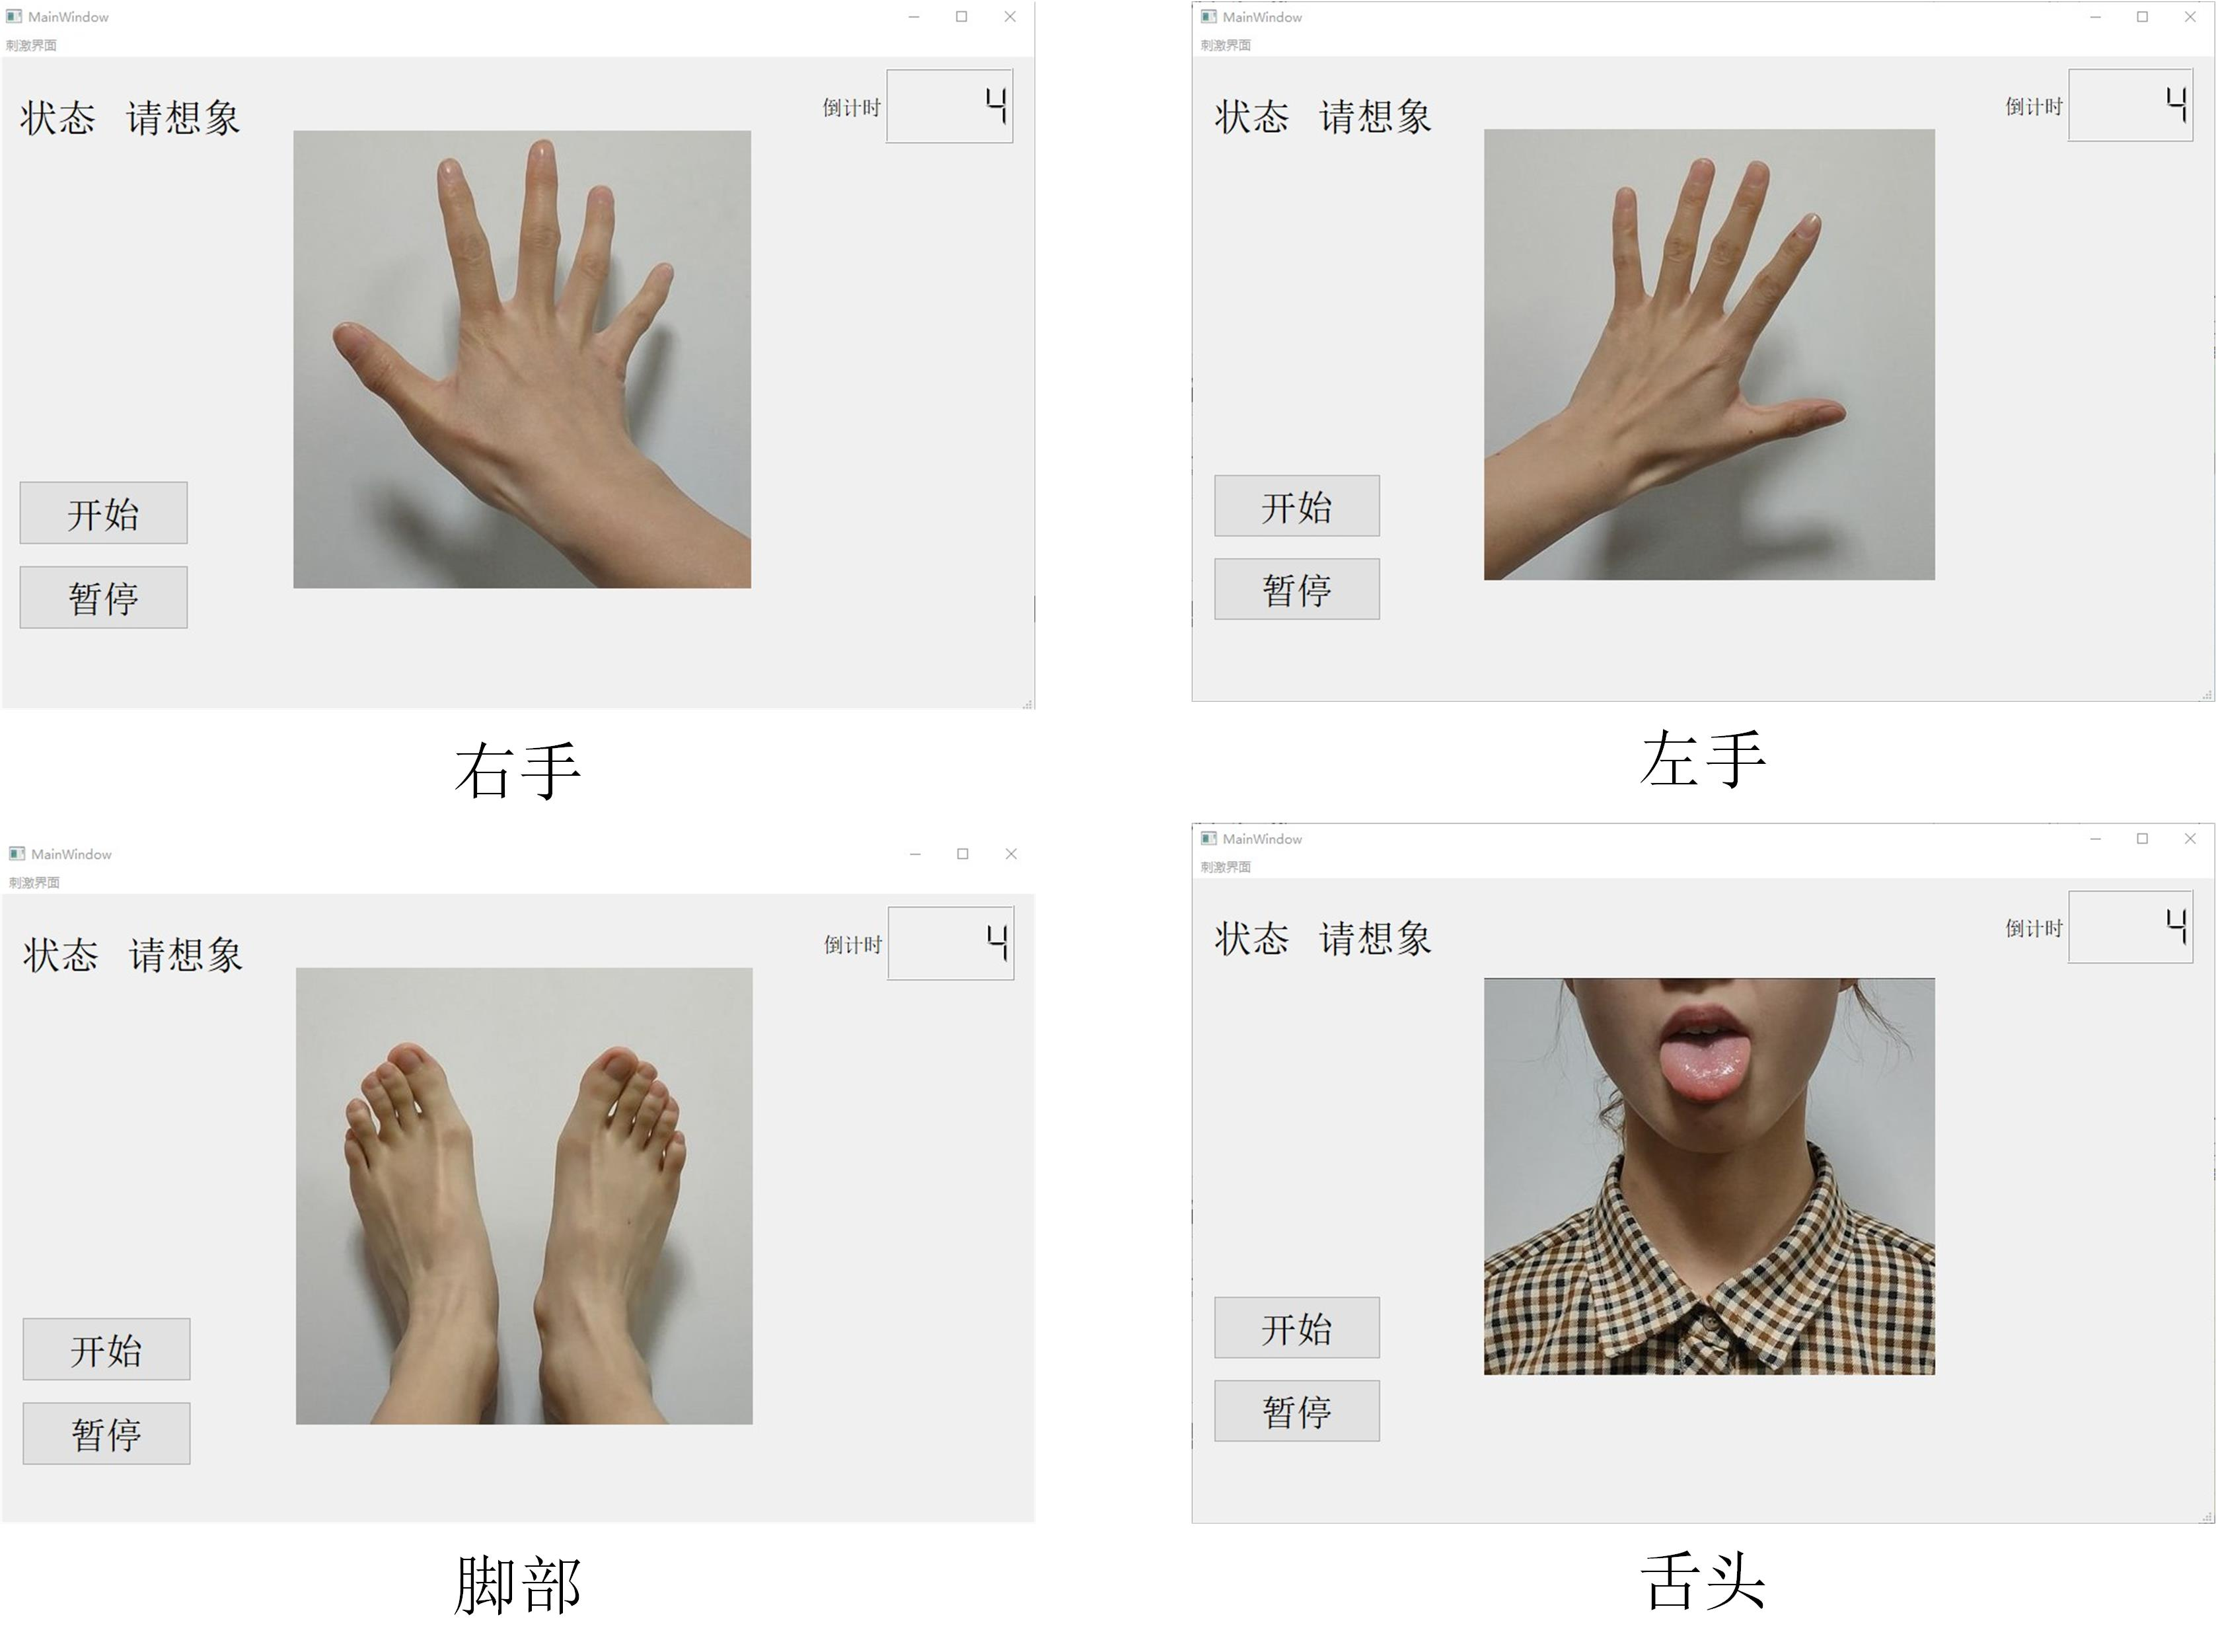
\includegraphics[width=0.57\textheight]{figures/运动想象实验.jpg}
	\caption{提示界面} 
	\label{fig_4_3}
\end{figure}

实验结束后,首先与BCI IV IIa数据集一致,进行0.5 Hz-100 Hz的带通滤波。紧接着,将数据下采样至250 Hz。为了去除可能存在的眼电干扰,使用独立分量分析\cite{4-29}对EEG数据进行处理。最后,参照Brunner等人研究\cite{4-10}中的描述,本章节仅保留JS-AINS-40的40个通道中与BCI IV IIa相同或位置相近的22个完成分类任务,具体为:Fz, FT7,FC3,FCz,FC4,FT8,T7,C3,Cz,C4,T8,TP7,CP3,CPz,CP4,TP8,P7,P3,Pz,P4,P8,Poz。

% IIA 原始通道:Fz, FC3, FC1, FCz, FC2, FC4, C5, C3, C1, Cz, C2, C4, C6, CP3, CP1, CPz, CP2, CP4, P1, Pz, P2, Poz。



\subsection{对比方法}
本文引入八种先进的算法进行结果对比,包括ShallowConvNet\cite{4-11}、EEGNet\cite{4-2}、EA-CSP\cite{4-15}、DRDA\cite{4-16}、MS-MDA\cite{4-17}、DAAN\cite{4-18}、CDAN\cite{4-19}和MCC\cite{4-20}。上述比较方法涉及机器学习算法、经典的深度学习模型和无监督域适应算法。这些算法中的大多数已经被证明可以胜任MI分类任务。考虑到本章所提出的模型属于无监督域适应的一种,上述对比方法中还包括了基于对抗策略、基于多源域和基于条件对齐的无监督域适应算法,以此证明本模型在无监督域适应领域中的先进性。

(1) ShallowConvNet(S-Conv)

一个专门为提取振荡信号中对数功率谱相关特征而设计的卷积网络结构。ShallowConvNet由连续的时间空间模块、非线性激活函数和全连接层组成。

(2) EEGNet

一个紧凑的卷积神经网络,设计了一种经典的EEG特征提取结构。深度卷积和可分离卷积的引入使其能够在不同范式的各种EEG信号上获得有竞争力的结果。在本文中,EEGNet-8,2被进行调整以适应250 Hz采样率的EEG信号。具体来说,EEGNet的第一个二维卷积核从(1,64)改为(1,125);第一个二维平均池化层从(1,4)改为(1,8)。

(3) EA-CSP

一种被广泛应用于MI-EEG场景下的迁移学习框架,它有效地结合了欧氏空间对齐和多分类CSP模型。本文引入线性判别算法(Linear Discriminant Analysis,LDA)对EA-CSP中提取的特征进行分类。

(4) DRDA

一种针对MI-EEG信号的新型端到端深度域适应方法,可以利用不同被试的判别性潜在特征提高分类性能。DRDA采用的中心损失技术可以进一步降低特征空间的非平稳性。由于其代码未公开,本文仅给出BCI IV IIa上的结果。

(5) MS-MDA

作为一种全新的迁移学习框架,MS-MDA为来自多个不同源域的EEG数据分别构建了独立的分支,用一对一的域适应方法来对齐多源域的边缘分布。由于该模型为情绪EEG设计,在本文中其通用特征提取器(Common Feature Extractor)被替换为MTSF以确保比较的公平性。同时,在MTSF和特定域特征提取器(Domain-specific Feature Extractor)之间加入了一个全连接层,以保证特征维度的一致性。

(6) DAAN

DAAN同时考虑了边缘分布(全局分布)和条件分布(局部分布)的贡献差异。它引入了动态学习来定量评估全局和局部域分布的相对重要性。使用MTSF作为DAAN的特征提取器。

(7) CDAN

CDAN是一个基于对抗的域适应方法,其将对抗学习与分类器预测中获取的鉴别性信息进行结合。在CDAN中,多线性调节(Multilinear Conditioning)被用来捕捉特征表示和分类器预测之间的交叉协方差。熵调节(Entropy Conditioning)被用来控制分类器预测的不确定性并确保模型具有足够的迁移能力。同样地,MTSF被引入作为CDAN的特征提取器。

(8) MCC

MCC提出了一个全新的损失函数,可以胜任多种迁移任务。这是一种具有快速收敛性的非对抗性域适应方法。它的性能已经在多源部分域适应(Multi-source Partial Domain Adaptation)和多目标部分域适应(Multi-target Partial Domain Adaptation)中得到了证明。这里,MTSF被用作特征提取器。

\subsection{实验设定}

由于所提出的模型是为多被试场景而设计的,使用LOSO对模型进行训练与测试。来自一个被试的数据被选为测试集(目标域),所有其他被试被视为训练集(源域)。为了充分验证模型在实际应用中的性能,本文设计了一个严苛的BCI系统使用场景,即训练数据和测试数据既不是来自同一被试,也不是来自同一时段。所有的对比方法也都遵循上述设定。值得注意的是,本文关于Additional Dataset的实验方案遵循了数据集作者所提出的“Subject-Independent”设置\cite{4-12, 4-13}。

本章所提出的模型和对比方法中的域适应算法直接利用了数据集所提供的预处理数据,没有进行额外的滤波操作。但是为了公平起见,对S-Conv、EEGNet和EA-CSP三种经典模型的输入数据额外进行了带通滤波处理。具体参数设定遵循 Chen等人\cite{4-21}、 Schirrmeister等人\cite{4-11}和Zhang等人\cite{4-13}的相关工作,对BCI IV IIa Dataset和JS-MI Dataset进行3-40 Hz的带通滤波,对High Gamma Dataset使用3 Hz-124 Hz的带通滤波,对Additional Dataset使用8 Hz-30 Hz的带通滤波。BCI IV IIa Dataset、JS-MI Dataset和High Gamma Dataset采用三阶巴特沃斯滤波器,而Additional Dataset采用五阶巴特沃斯滤波器。

所提出的方法基于AMD CPU(R9-3950X,3.5 GHz)和NVIDIA GPU(RTX 3090)在Pytorch中实现。其使用Adam优化器,将动量设置为0.9,学习率设置为0.001。根据数据集的大小,BCI IV IIa Dataset、JS-MI Dataset、High Gamma Dataset和Additional Dataset的权重衰减分别被设置为0.001、0.001、0.0006和0.0005。batch size的大小被设定为64,一个训练阶段的epoch数量设定为300。除了固定随机种子以外,在深度神经网络基元库cuDNN中,deterministic被设置为True,benchmark被设置为False,以保证每次运行使用默认卷积算法,确保算法复现性。所有对比方法的参数均在其原始代码的基础上,根据不同MI数据集进行了单独调整,以保证比较的公平性。所有比较方法的batch size和epoch都被设定为64和300。

(1) S-Conv与EEGNet

对于S-Conv和EEGNet,其学习率被设置为0.001。对于BCI IV IIa Dataset、JS-MI Dataset、High Gamma Dataset和Additional Dataset,权重衰减分别被设置为0.01、0.01、0.005和0.001。S-Conv和EEGNet均采用Adam优化器,动量设置为0.9。

(2) EA-CSP

对EA-CSP,设定其CSP空间滤波器个数为3。

(3) MS-MDA

对MS-MDA,设置学习率为0.001。根据其原始代码中的设置,其没有引入权重衰减。采用Adam优化器,动量设置为0.9。

(4) DAAN

对于DAAN,学习率被设置为0.001。BCI IV IIa Dataset、JS-MI Dataset、High Gamma Dataset和Additional Dataset的权重衰减被设置为0.001、0.001、0.0006和0.0005。采用SGD优化器,动量为0.9。

(5) CDAN

对于CDAN,设置学习率为0.01,学习率衰减为0.1。对于BCI IV IIa Dataset、JS-MI Dataset、High Gamma Dataset和Additional Dataset,权重衰减分别设置为0.001、0.001、0.0006和0.0005。CDAN引入了动量为0.9的SGD优化器。同时,考虑到特征提取器(MTSF)的输出维度,本文采用了CDAN提出的全线性条件预测(Full-bilinear Conditional Predictions)。

(6) MCC

对于MCC,将学习率设置为0.001。对于BCI IV IIa Dataset、JS-MI Dataset、High Gamma Dataset和Additional Dataset,权重衰减被设置为0.001、0.001、0.0006和0.0001。此外,采用Adam优化器,动量设置为0.9。



\section{实验结果}
\subsection{分类结果}
从LOSO实验中得到的平均辨识准确率见表\ref{tab4-2}。此外,威尔科克森符号秩检验(Wilcoxon Signed Rank Test)的$P$值被用来衡量所提出的模型和其他基线之间准确率的显著差异\cite{4-28}。表\ref{tab4-2}中的星号表示显著差异的程度,可以看出,ISMDA优于所有的比较方法,并且均具有统计学意义上的显著性差异($p < 0.05$)。

\begin{table*}[!h]
\caption{所有被试的平均分类准确率(\%)}  \label{tab4-2}
\centering
\wuhao{
  \begin{threeparttable}
  \setlength{\tabcolsep}{0.8mm}{
    \begin{tabular}{cccccccccc}
        \toprule
        \multirow{2}*{\textbf{数据集}}    &  \multicolumn{9}{c}{\textbf{算法}} \\
                            \cline{2-10} 
					      \specialrule{0em}{0pt}{0pt}
                           &S-Conv &EEGNet  &EA-CSP   &DRDA  &MS-MDA   &DAAN  &CDAN  &MCC   &\textbf{ISMDA} \\    
        \midrule
        BCI IV IIa    &\multirow{2}*{47.92$^{**}$}   &\multirow{2}*{48.51$^{**}$} &\multirow{2}*{39.27$^{**}$} &\multirow{2}*{52.92} &\multirow{2}*{55.84$^{**}$} &\multirow{2}*{62.22$^{**}$} &\multirow{2}*{63.82$^{*}$} &\multirow{2}*{66.51$^{*}$} &\multirow{2}*{69.51} \\
        Dataset &&&&&&&&& \\       
        High Gamma              &\multirow{2}*{70.56$^{***}$}   &\multirow{2}*{60.83$^{***}$} &\multirow{2}*{56.98$^{***}$} &\multirow{2}*{-}     &\multirow{2}*{77.09$^{***}$} &\multirow{2}*{77.62$^{**}$} &\multirow{2}*{78.34$^{**}$} &\multirow{2}*{81.24$^{*}$} &\multirow{2}*{82.38}\\
        Dataset &&&&&&&&& \\
        Additional &\multirow{2}*{75.44$^{***}$} &\multirow{2}*{69.71$^{***}$} &\multirow{2}*{64.25$^{***}$} &\multirow{2}*{-}     &\multirow{2}*{57.67$^{***}$} &\multirow{2}*{80.44$^{***}$} &\multirow{2}*{89.49$^{**}$} &\multirow{2}*{85.61$^{***}$} &\multirow{2}*{90.98}\\
        Dataset &&&&&&&&& \\ 
        JS-MI     &\multirow{2}*{52.91$^{**}$} &\multirow{2}*{55.65$^{**}$} &\multirow{2}*{43.75$^{**}$} &\multirow{2}*{-} &\multirow{2}*{60.10$^{**}$} &\multirow{2}*{65.35$^{*}$} &\multirow{2}*{67.43$^{*}$} &\multirow{2}*{68.58$^{*}$} &\multirow{2}*{70.08}\\
        Dataset &&&&&&&&& \\ 
        \bottomrule
    \end{tabular}
    }
    \begin{tablenotes}
	    \footnotesize
        \item 威尔科克森符号秩检验:$p < 0.05$:$^*$,$p < 0.01$:$^{**}$,$p < 0.001$:$^{***}$。
        \item -:代码未开源,没有相关数据。
    \end{tablenotes}
  \end{threeparttable}}
\end{table*}

(1) BCI IV IIa Dataset

由表\ref{tab4-2}可以看出,基于特征提取器EA-CSP与机器学习分类器LDA组成的模型取得了最差的分类结果。简单的遵循特征提取器加机器学习分类器的模型设计思路,已经无法获得具有足够跨域泛化能力的模型,难以应对本文所面临的应用场景。两种常见的基于深度学习算法的EEG分类模型S-Con和EEGNet,取得了比EA-CSP更好的结果,但其性能远逊于深度域适应模型。以DRDA为代表的域适应算法极大地提高了分类任务的最终准确率,这表明当不同域之间的偏差很大时,能够有效提取潜在空间的域不变表征的算法将具有更高的迁移能力。尤其可以看到,DAAN、CDAN、MCC和ISMDA可以达到领先于经典EEG辨识模型15\%-20\%的优异结果。从统计学的角度来看,ISMDA相较于大多数基线模型具有明显的优势,并以至少0.05的显著性水平超过了两个极具竞争力的对比方法CDAN与MCC。 

(2) High Gamma Dataset

凭借高质量的采集条件和较短的采集时间间隔,High Gamma Dataset让所有模型都在其上取得了较高的辨识精度。然而,与BCI IV IIa Dataset相比,所有方法最终性能的排序并没有发生明显变化,这验证了上文对各个模型特征的分析。其中,MS-MDA、DAAN、CDAN和MCC仍然取得了极为优异的结果,这也进一步证明了MTSF的有效性。尽管对比算法中的域适应方法和ISDMA在High Gamma Dataset上的平均准确率差异并不显著,但由于受试者数量的增加,ISMDA在统计学对比上仍占据优势。

(3) Additional Dataset

由于Additional Dataset具有更多受试者和较少的MI类别,大多数方法在其上都获得了较高的分类精度。然而,MS-MDA的性能却产生了显著下降,这主要是由以下原因造成。首先,MS-MDA需要对所有源域和目标域进行对齐,当受试者数量变多时,这极易造成训练过程的不收敛。其次,MS-MDA建立在源域中的每个被试与目标域中的被试拥有相同数据量的前提下。而在本章中,Additional Dataset上的LOSO实验遵循了Kwon等人\cite{4-12}与Zhang等人\cite{4-13}的设定,因此目标域的被试仅使用了其第四个时段的样本。同时,ISMDA的提出是为了建立一个具有高度泛化能力的模型,它不能要求每个被试均具有相同规模的数据量。MS-MDA的性能下降,表明其不能适应这种应用环境。在BCI IV IIa Dataset和High Gamma Dataset上极具竞争力的MCC在Additional Dataset上变得不再强势,这主要是因为Additional Dataset只包含两个类别。MCC以区分易混淆的类别为目标来提升模型性能,而较少的类别使其无法发挥优势。在有更多受试者的Additional Dataset上,ISMDA以压倒性的高显著性水平优于所有对比方法,这证实了它在不同数据集上的鲁棒性。

(4) JS-MI Dataset

JS-MI Dataset采用了与BCI IV IIa Dataset相同的实验流程,并且数据集规模也保持一致。因此所有方法在二者上取得了相近的结果。然而,可以明显看出,所有方法在JS-MI Dataset上均取得了更好的辨识结果,这很可能归功于采集设备性能的提升。特别是在经典的EEG辨识模型——S-Conv、EEGNet与EA-CSP上,JS-MI Dataset具有更大幅度的性能增长,这意味着在JS-MI Dataset上有效的MI分类特征更加容易被获取。诚然,JS-MI Dataset带来的性能变化很可能来自于很多方面,比如较低的EEG文盲比例(44.4\%)、更高质量的采集环境以及其他不可控的外在因素等。但是毫无疑问,JS-MI Dataset证明了JA-AINS-40系统具有足够可靠的性能。

\begin{table*}[!h]
\caption{ISMDA不同变体的分类性能(\%)}  \label{tab4-3}
\centering
\wuhao{
    \begin{threeparttable}
    \setlength{\tabcolsep}{1.1mm}{
        \begin{tabular}{ccccccc}
            \toprule
            \multirow{3}*{\textbf{数据集}}   &  \multicolumn{6}{c}{\textbf{算法}} \\ 
            \cline{2-7} 
		\specialrule{0em}{0pt}{0pt}
            
                               &\textbf{SourceCNN} &\textbf{ISMDA}   &\textbf{ISMDA}    &\textbf{ISMDA}     &\textbf{ISMDA}    &\textbf{ISMDA} \\    
            % \Xcline{1-15}{0.4pt}
                               &\textbf{(MTSF)}    &\textbf{w/o DAM} &\textbf{w/o DCIS} &\textbf{w/o ATDOC} &\textbf{w/o PACC} &\\
            \midrule
            BCI IV IIa Dataset &50.36     &65.57   &63.63    &64.69     &67.27    &69.51 \\
            High Gamma Dataset &65.14     &79.35   &80.67    &80.99     &81.33    &82.38\\
            Additional Dataset &75.97     &88.59   &89.42    &90.14     &90.57    &90.98\\
            JS-MI Dataset      &58.29     &67.54   &66.15    &66.93    &69.20    &70.08\\
            \bottomrule
        \end{tabular}
        }
    \end{threeparttable}
    }
\end{table*}

此外,ISMDA的不同变体,包括SourceCNN(即只包含MTSF),去掉DMA(ISMDA w/o DAM),去掉DCIS(ISMDA w/o DCIS),去掉ATDOC(ISMDA w/o ATDOC)以及去掉PACC(ISMDA w/o PACC)的辨识结果已经在表格\ref{tab4-3}中给出,本文在章节4.4对其内容进行了详细分析。


\subsection{算法复杂度}

本章对所有算法的训练时间消耗以及参数数量进行了详细比较,如表\ref{tab4-4}所示。从总体上看,经典的深度学习模型以及机器学习模型对于计算资源的消耗远低于无监督域适应算法。并且,所有的无监督域适应算法的计算时间均处于同一数量级。

\begin{table*}[!h]
\caption{每名被试所需要的平均训练时间和所有方法的可训练参数数量}  \label{tab4-4}
\centering
\wuhao{
\begin{threeparttable}
 \setlength{\tabcolsep}{1mm}{
    \begin{tabular}{ccccccc}
        \toprule
        \multirow{3}*{\textbf{算法}}         & \multicolumn{2}{c}{\textbf{BCI IV IIa Dataset}}  & \multicolumn{2}{c}{\textbf{High Gamma Dataset}} & \multicolumn{2}{c}{\textbf{Additional Dataset}}\\
    
        \cline{2-7}
        \specialrule{0em}{0pt}{0pt}
                                   & 时间消耗 & 参数量     & 时间消耗 & 参数量 
                                   & 时间消耗 & 参数量\\
                                   & (GPU-hours)      & (M)        & (GPU-hours)      & (M)    
                                   & (GPU-hours)      & (M)     \\
        \midrule
       
        S-Conv             & 0.34             & 0.013764   & 1.18             & 0.432164   & 2.70             & 0.305282\\
 
        EEGNet                     & 0.28             & 0.003992   & 1.06             & 0.005400   & 2.78             & 0.006072 \\
        
        EA-CSP                     & 0.01             & /          & 0.03             & /          & 0.07             & /         \\
       
        SourceCNN(MTSF)           & 0.40             & 0.369224   & 1.23             & 0.373448   & 3.31             & 0.375902 \\
      
        MS-MDA                     & 1.32             & 0.071072   & 5.83             & 0.086676   & 10.14            & 0.177674 \\
     
        DAAN                       & 0.84             & 3.442494   & 2.47             & 3.446718   & 6.88             & 2.221730 \\
    
        CDAN                       & 0.72             & 0.372105   & 1.89             & 0.376329   & 6.05             & 0.377343 \\
     
        MCC                        & 0.81             & 0.369224   & 1.47             & 0.373448   & 6.01             & 0.375902 \\
        
        ISMDA w/o DAM              & 1.20             & 0.369224   & 3.46             & 0.373448   & 6.83             & 0.375902 \\
        
        ISMDA w/o DCIS             & 0.43             & -          & 1.29             & -          & 3.34             & -       \\
        
        ISMDA w/o ATDOC            & 1.29             & -          & 3.38             & -          & 6.84             & -       \\
        
        ISMDA w/o PACC             & 0.86             & -          & 1.66             & -          & 3.41             & -       \\
     
        ISMDA                      & 1.36             & 1.483172   & 3.57             & 1.487396   & 6.92             & 1.489850 \\
        \bottomrule
    \end{tabular}
    }
    \begin{tablenotes}
	    \footnotesize
	    \item GPU-hours:在一块RTX 3090上运行得到。
	    \item /:无可训练参数。
	    \item -:与ISMDA的结果相同。
    \end{tablenotes}
\end{threeparttable}
}
\end{table*}

具体来说,EA-CSP由于缺乏可训练的参数,其计算消耗最小。S-Conv、EEGNet和SourceCNN (MTSF)由于其方法和结构的相似性,训练时间几乎相同。由于SourceCNN (MTSF)的多分支结构和其分类器的复杂性(比S-Conv、EEGNet多一层全连接层),其参数数量较多。MS-MDA要求源域的所有受试者与目标域的受试者分别进行对齐,这导致了计算时间随着受试者数量的增加而明显提升。DAAN为每个类别分别训练相应的判别器,这使它的参数数量远多于其他方法。CDAN和MCC几乎没有引入比MTSF更多的参数,并且它们的时间消耗也很低。CDAN的全线性条件预测使其参数量略多于MTSF。此外,MCC只引入了一个损失函数,因此它的计算资源消耗在所有的无监督域适应方法中最为亮眼。

对于ISMDA w/o DAM,其参数的数量相较于ISMDA有所减少,因为它改变了传递给分类器的特征尺寸。其余的ISMDA变体由于采用了相同的模型结构,其参数数量与ISMDA相同。可以注意到,DAM和ATDOC对训练时间的影响较小,而PACC由于引入了额外的训练阶段,几乎使训练时间增加了一倍。ISMDA比其他无监督域适应方法拥有更多的参数,然而它们的计算时间消耗基本处于同一水平。据此认为,ISMDA的计算资源消耗仍处于可接受的水平。特别的是,当被试数量增加时,ISMDA变得更有竞争力。

综上分析,同一算法在不同数据集上的计算资源消耗主要取决于数据集的数据规模,具体来说包括:被试人数,每名被试的试验次数,每次实验采集数据的EEG通道数,采样点数以及MI类别数。然而,JS-MI Dataset因为遵循与BCI IV IIa Dataset完全相同的实验流程,对于上述影响计算复杂度的因素,二者完全一致。理论上不同算法在JS-MI Dataset与BCI IV IIa Dataset上的训练时间消耗以及可训练参数数量完全相同,因此,本章在表\ref{tab4-4}中没有再增加JS-MI Dataset的相关内容。值得注意的是,表\ref{tab4-4}中的结果与机器特性高度相关,只能作为参考。


\section{消融实验}
在本节中,通过以下实验探讨了ISMDA的三个组成部分的重要性以及其超参数的合理性。本章所涉及的所有消融实验均基于LOSO原则,以确保消融结果和参数分析的合理性。
\subsection{平行滤波器的可视化}
MTSF模块包含三组针对MI-EEG域特征所设计的组合式时空滤波器。已有的研究表明\cite{4-22},当人脑想象身体运动时,相应的皮质映射区域会出现EEG的节律调节现象,即ERD或ERS\cite{4-23}。当想象左手或右手的运动时,其对侧脑半球区域的生理电信号活跃度上升,该区域对这些信息的处理会导致其功率谱密度降低。相应的,在进行脚和舌头的运动想象时,这一现象将分别出现于顶叶和颞叶。

\begin{figure*}[!h]
\centering
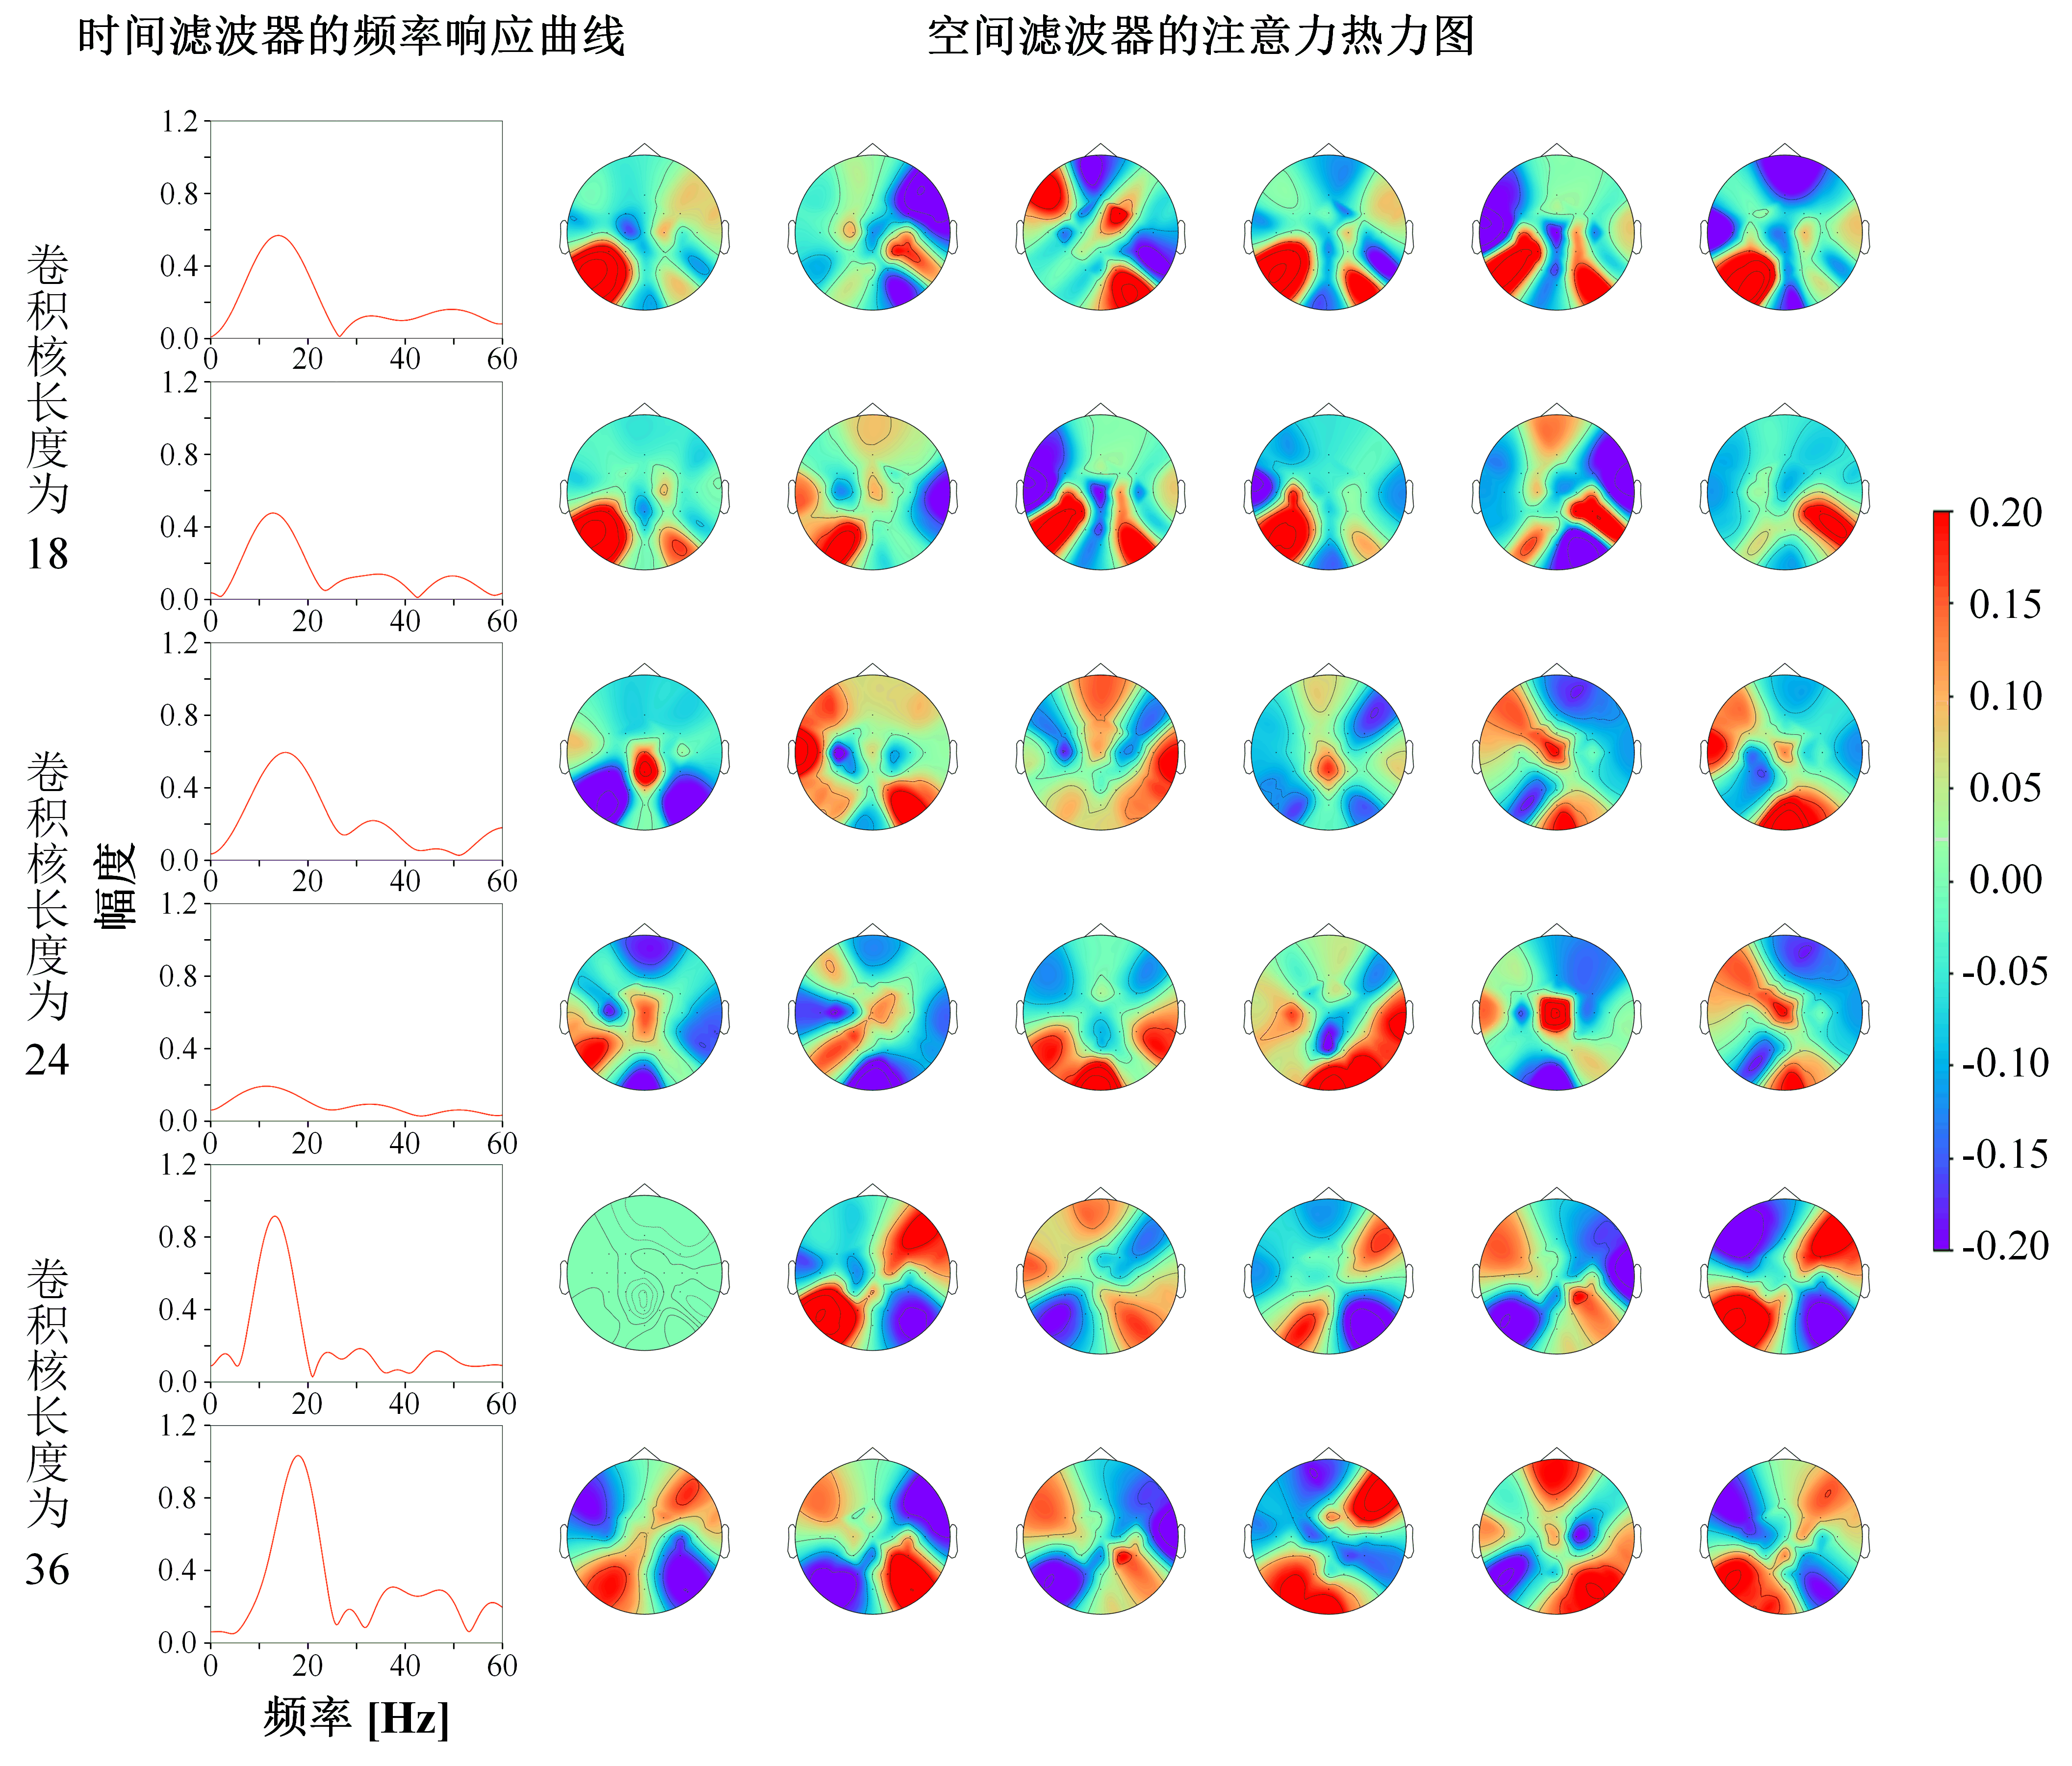
\includegraphics[width=1.0\textwidth]{topmap.png}
\caption{随机选择的两个时间滤波器的频率响应,以及连接在它们后面的空间滤波器注意力热力图。}
\label{fig_4_4}
\end{figure*}

在不同的MI任务中,激活的脑区的空间分布与周围神经纤维和大脑皮层之间的投影关系一致,这在大脑的功能分区理论中也得到了印证。因此,MI的EEG信号具有空间特征。同时,不同MI任务的ERD或ERS现象往往出现在不同的频段,手部常出现在10 Hz-15 Hz和20 Hz-24 Hz,脚部常出现在7 Hz-8 Hz和20 Hz-24 Hz,舌头常出现在10 Hz-11 Hz。此外,在频段特性上也存在一些个体差异\cite{4-24}。针对这一特点,本文设计了一个卷积核大小为18的时间滤波器来提取高频特征。根据所采用数据集的采样率,长度为18的卷积核可以针对性地提取14 Hz或以上频率的周期性信号特征,这与手部MI的频带一致。同样的,MTSF的另外两个分支分别提取10 Hz(卷积核大小为24)和7 Hz(卷积核大小为36)附近信号的频域特征,分别对应于舌头和脚的频段。为证明上述分析,随机在基于BCI IV IIa Dataset的ISMDA模型中挑选两组时空滤波器,并画出其频率响应和在大脑皮层上的空间注意力热力图。

在图\ref{fig_4_4}中,时间滤波器的频率响应证明了不同大小的卷积核能够实现网络对特定频段关注的推论。同样可以看到,针对左手和右手的空间滤波器显然在C3和C4电极附近投入了更多的注意力,而脚的空间滤波器在头皮两侧的颞叶附近拥有更高的权重。同时,针对舌头的空间滤波器在顶叶和颞叶附近都具有较高的激活度。

上述结果与人脑的生理特性\cite{4-24}一致,证明了MTSF设计的可靠性。也说明了在MTSF的基础上,针对不同运动想象动作的时频域以及空间特征进行模型搭建,是可行且合理的。


\subsection{动态注意力模块的影响}
为了进一步探索DAM的有效性,本章从四个方面分析了DAM带来的影响。分别是分类精度、域间差异、特征分布以及超参数选取。

(1) 分类精度

为了直观地比较不同模块带来的影响,表\ref{tab4-3}和表\ref{tab4-5}中介绍了ISMDA变体的更多分类结果。表\ref{tab4-3}比较了DAM对所有数据集的最终辨识精度的影响。相较之下,表\ref{tab4-5}则显示了High Gamma Dataset上每个类别的分类精度以及最显著的类别间错误分类概率。MS-MDA、DAAN、CDAN和MCC与不同的特征提取器进行了配对,用来进一步比较特征提取器间性能的差异性。如表\ref{tab4-3}所示,DAM的引入提高了MTSF寻找域不变表征的能力,使模型的解码性能从与EEGNet相似提高到了与CDAN接近。然而,从表\ref{tab4-5}中的ISMDA w/o DCIS也可以看出,在High Gamma Dataset上的左手和右手类别之间存在着严重的偏向性,这说明DAM的引入偏移了模型的判别能力。特别的是,在左手和右手之间,右手更容易被模型选中。这种现象可能是由于High Gamma Dataset中的被试大部分为右利手,他们长期使用右手的习惯使他们在进行右手MI时更容易产生相应的ERD或ERS反应。此外,由于卷积核长度为18的时间滤波器同时提取了右手和左手特征,二者之间必然会存在一些混杂。因此,DAM倾向于在用大量数据训练后,从混杂的样本中动态迁移具有相对更明显特征的右手样本。同样的,对右手的青睐也出现在其他可比较的模型中,在大多数情况下,将左手错误分类为右手的概率比反之高大约5\%。
\begin{table*}[!t]
\caption{High Gamma Dataset上的分类辨识实验结果\label{tab4-5}}
\centering
\wuhao{
\begin{threeparttable}
\setlength{\tabcolsep}{1.8mm}{
    \begin{tabular}{ccccccccc}
        \toprule
        \multirow{3}*{\textbf{算法}}   & \multicolumn{4}{c}{\textbf{准确率(\%)}} & \multicolumn{4}{c}{\textbf{误判率(\%)}}\\
        \cline{2-9}
                           & \multirow{2}*{\textbf{左手}} & \multirow{2}*{\textbf{右手}} & \multirow{2}*{\textbf{休息}} & \multirow{2}*{\textbf{舌头}} & \textbf{左手} &\textbf{右手} 
                           &\textbf{休息} &\textbf{舌头}\\
                           &&&&&\textbf{$\Rightarrow$右手}&\textbf{$\Rightarrow$左手}&\textbf{$\Rightarrow$舌头}&\textbf{$\Rightarrow$休息}\\
        
        \midrule
        \multicolumn{9}{c}{\textbf{传统算法}}\\                  
        \midrule
        S-Conv              & 68.51 & 	67.86 & 71.43 & 74.44 & 24.55 & 20.63 & 11.76 & 13.59 \\
        EEGNet                     & 56.83 & 	59.77 & 62.32 & 64.40 & 27.61 & 22.39 & 12.84 & 15.45 \\
        EA-CSP                     & 55.43 & 	56.16 & 57.29 & 59.04 & 26.41 & 25.17 & 18.13 & 20.40 \\
        SourceCNN(MTSF)           & 62.53 & 	64.78 & 67.28 & 65.97 & 25.82 & 20.73 & 12.55 & 14.98 \\
        \midrule
        \multicolumn{9}{c}{\textbf{域适应算法}}\\ 
        \midrule
        MS-MDA+S-Conv   & 74.67 & 	77.58 & 76.12 & 73.75 & 22.34 & 17.77 & 14.15 & 17.70 \\
        MS-MDA+EEGNet           & 71.86 & 	75.77 & 76.95 & 73.10 & 25.64 & 16.31 & 13.57 & 18.85 \\
        MS-MDA+MTSF & 73.94 & 	78.13 & 77.86 & 78.51 & 23.45 & 15.93 & 12.81 & 16.38 \\
        DAAN+S-Conv       & 75.52 & 	77.03 & 76.36 & 80.61 & 22.93 & 17.97 & 12.52 & 13.49 \\
        DANN+EEGNet                   & 72.71 & 	74.88 & 76.82 & 79.51 & 24.52 & 16.79 & 13.83 & 14.97 \\
        DANN+MTSF         & 74.50 & 	77.35 & 79.19 & 79.45 & 21.58 & 17.13 & 11.84 & 13.25 \\
        CDAN+S-Conv           & 77.64 & 	79.30 & 80.75 & \textbf{82.75}  & 18.41 & 14.97 & 9.10  & 13.52 \\
        CDAN+EEGNet                   & 73.68 & 	75.13 & 76.24 & 77.71 & 24.11 & 17.07 & 10.72 & 17.85 \\
        CDAN+MTSF         & 77.16 & 	77.10 & 83.12 & 76.01 & 16.76 & 15.54 & 9.5   & 16.74 \\
        MCC+S-Conv      & 78.15 & 	79.48 & 81.32 & 82.20  & 16.11 & 14.50 & 9.94  & 13.91 \\
        MCC+EEGNet              & 75.36 & 	75.29 & 77.96 & 78.11 & 19.74 & 18.05 & 12.21 & 14.87 \\
        MCC+MTSF    & \textbf{80.19} & 	82.31 & 81.84 & 80.62 & \textbf{14.53} & 12.84 & 10.18   & 14.12 \\
        \midrule
        \multicolumn{9}{c}{\textbf{ISMDA及其变体}}\\ 
        \midrule
        ISMDA w/o DAM              & 78.13 & 	77.93          & 83.21           & 78.13 & 15.72 & 15.88 & 10.97  & 12.95 \\
        ISMDA w/o DCIS             & 75.18          & 	83.48          & 82.00           & 82.00 & 20.18          & 11.47          & 8.89  & \textbf{12.64} \\
        ISMDA w/o ATDOC            & 75.62          & 84.53              & 82.04           & 81.78 & 19.62          & 11.45          & 9.07  & 12.97 \\
        ISMDA w/o PACC             & 78.06          & 	\textbf{85.76} & 80.35           & 81.18 & 18.53          & \textbf{10.96} & 11.63 & 13.43 \\
        ISMDA                      & 77.79          & 	         84.17 & \textbf{85.85}  & 81.72 & 17.38          & 10.97          & \textbf{6.52}  & 12.75 \\
        \bottomrule
    \end{tabular}
    }
    \begin{tablenotes}
	    \footnotesize
	    \item 高亮的结果:每一列中的最优值。
	    \item 甲{$\Rightarrow$}乙:错误将甲判别为乙。
    \end{tablenotes}
\end{threeparttable}
}
\end{table*}

同时,由于频域和空间特征之间的相似性,在休息和舌头之间不可避免地存在着较高的误判概率。特别是,舌头的特征频率处于整个频段的中间位置,这使得它的特征更容易被误判。正如表\ref{tab4-5}所反映的,尽管模型可以根据空间分布特征将舌头与左(右)手区分开来,但它容易将舌头误判为休息。

(2) 域间差异

辨识性特征的域间差异是一个可以衡量模型可迁移性的重要指标。为了验证ISMDA的性能,本章引入了一个名为Global $\mathcal{A}$-distance\cite{4-25}的通用指标来准确测量域间差异。其公式如下:
\begin{equation}
\label{deqn_ex14}
\operatorname{Global\ dist}_{\mathcal{A}}\left(\mathcal{D}_{s}, \mathcal{D}_{t}\right)=2\left(1-2 \epsilon\right),
\end{equation}
其中$\operatorname{dist}_{\mathcal{A}}$代表了两个不同域之间的$\mathcal{A}$-distance,$\epsilon$代表了经过训练的二元分类器对源域和目标域中的样本进行域判别的错误率。遵循Ben-David等人\cite{4-25}的设定,针对每个被试的最优ISMDA模型被当作特征提取器,SVM被引入当作分类器。具体来说,为了计算一名被试的Global $\mathcal{A}$-distance,随机选取该名被试70\%的特征和与其等量的其他受试者的特征作为训练集来训练SVM。所有剩余的特征将被作为测试集来验证域间差异。这一过程对数据集中的所有受试者依次进行。通过对所有受试者的Global $\mathcal{A}$-distance进行平均,即获得了对该模型迁移性能的评估。从结果来看,Global $\mathcal{A}$-distance越小,证明ISMDA提取到的源域和目标域的特征越接近,这使得SVM更难对二者进行区分。如图\ref{fig_4_5}所示,ISMDA在所有数据集上均取得了最好的结果,而基于域适应的算法一般都比其他算法拥有更好的迁移性能。

\begin{figure*}[!t]
\centering
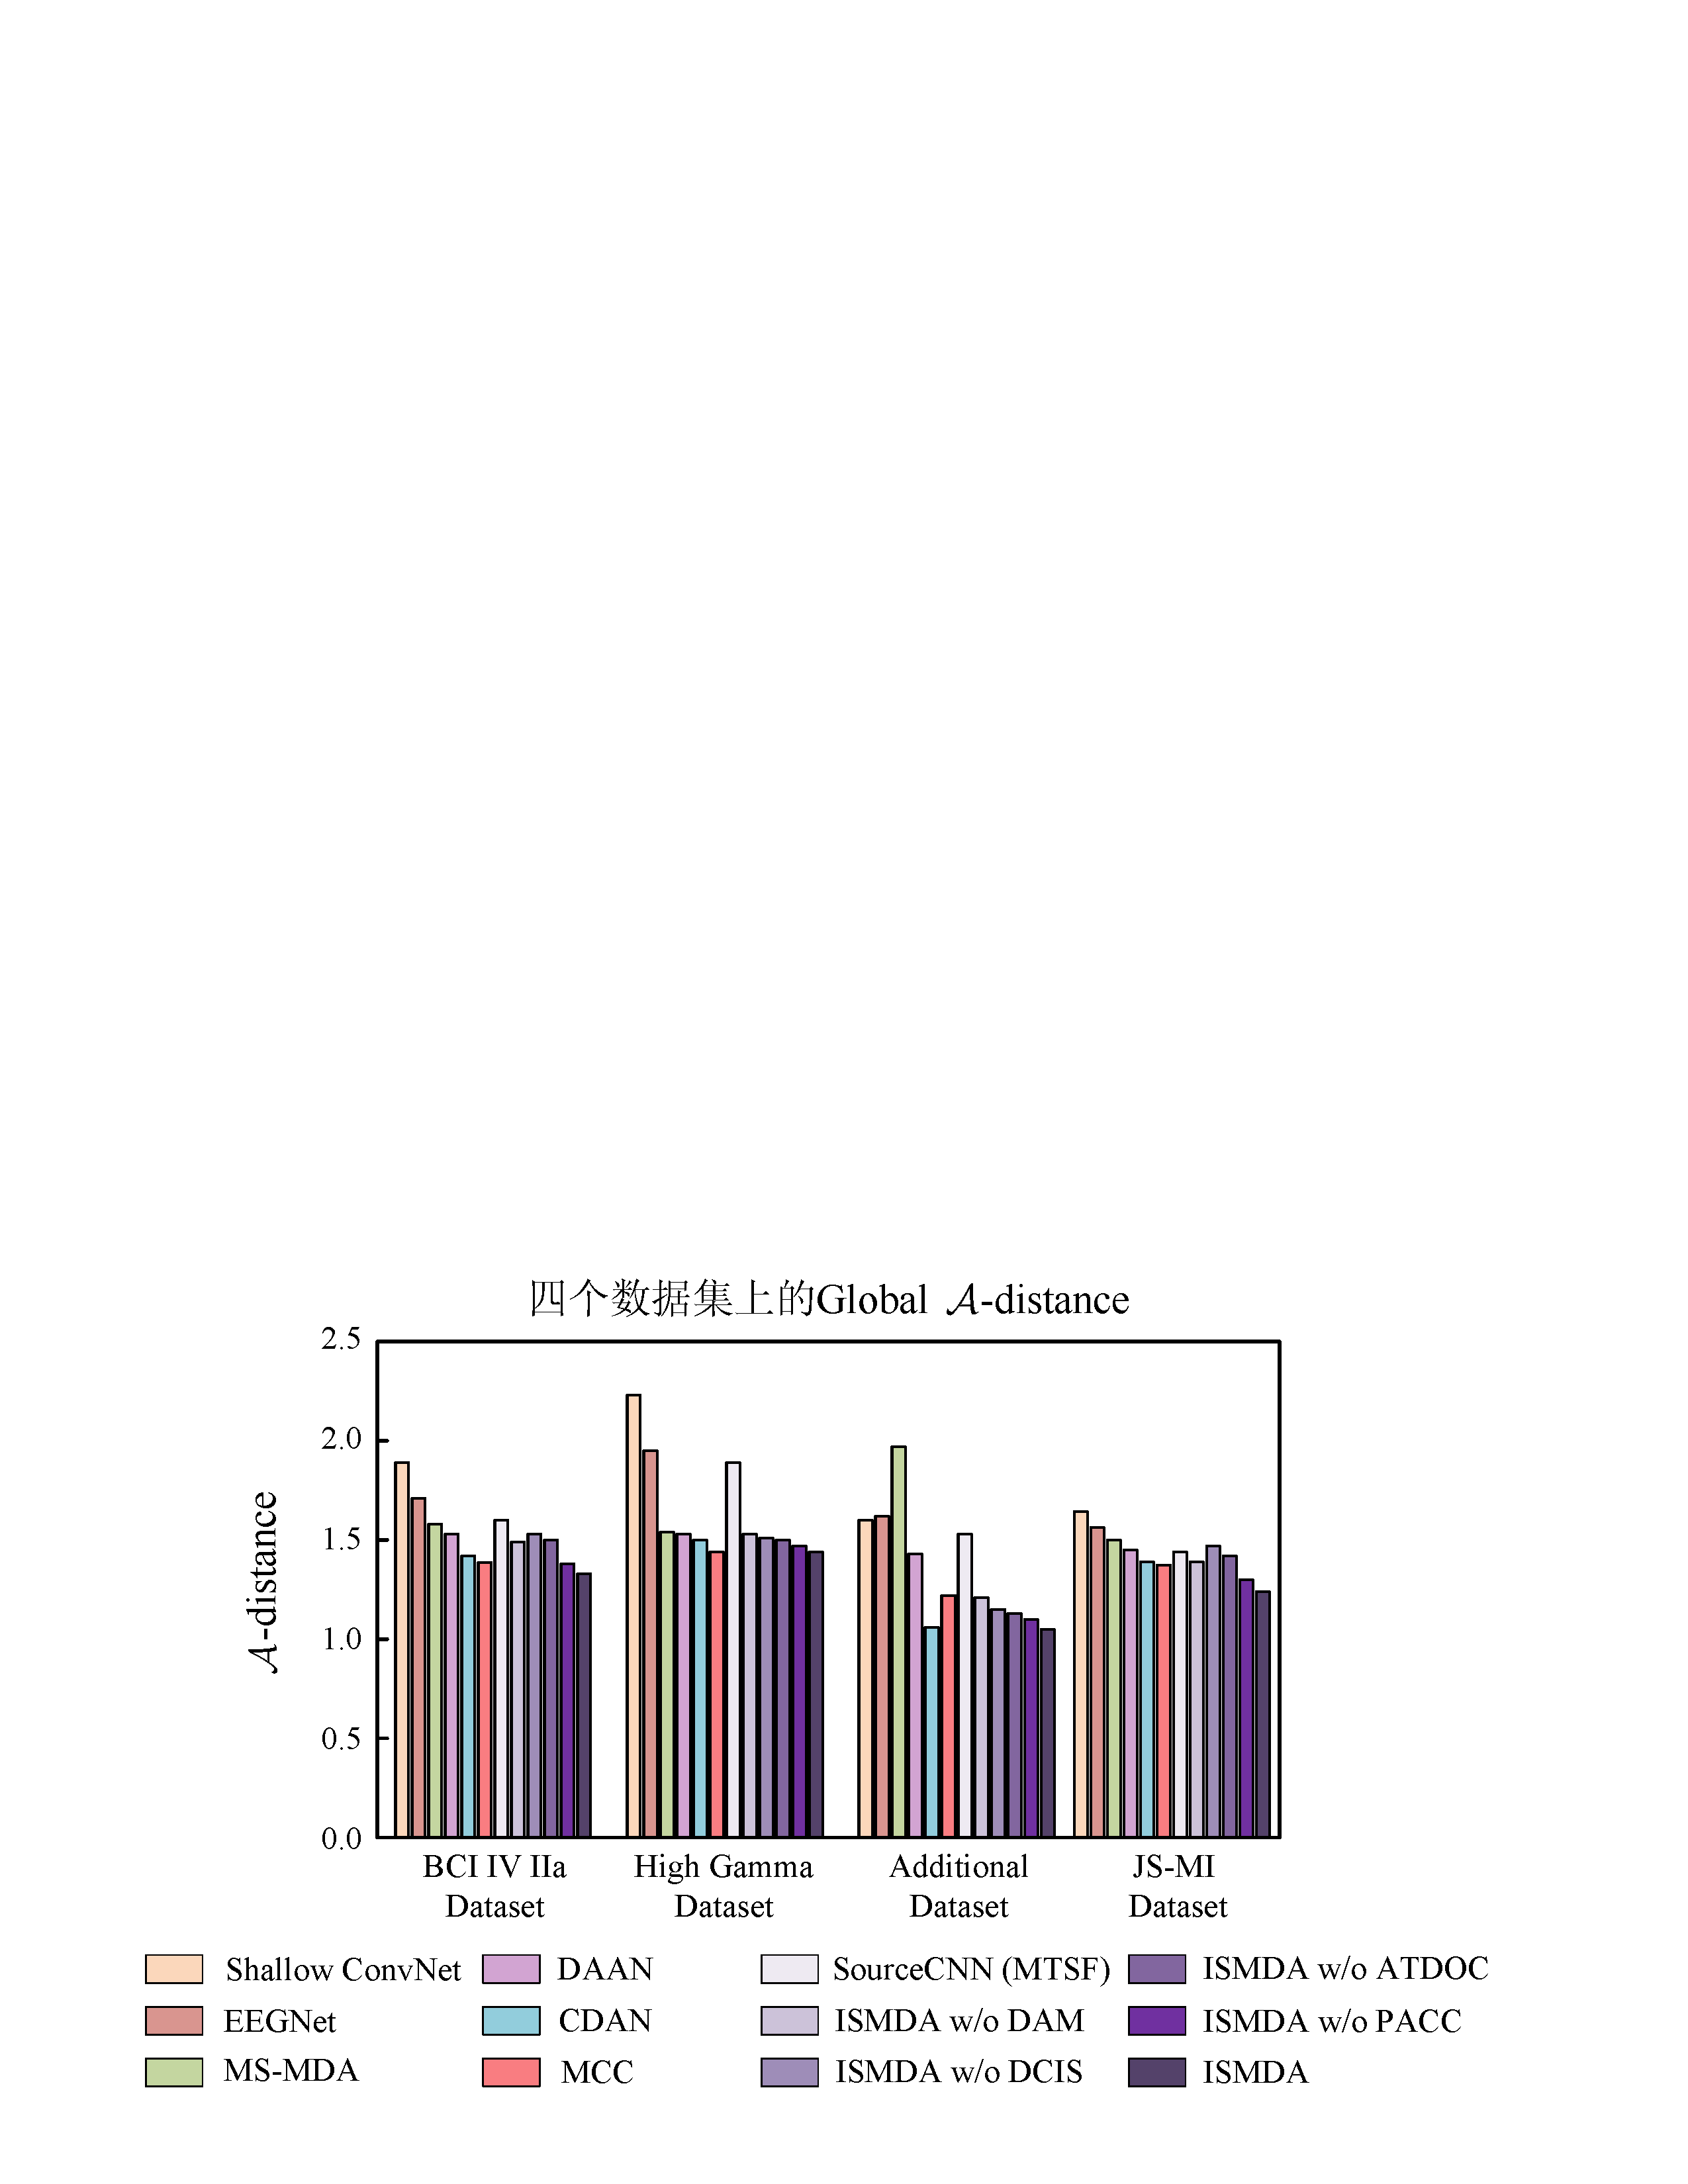
\includegraphics[width=0.90\textwidth]{A距离.pdf}
\caption{每个模型在所有数据集上的Global $\mathcal{A}$-distance(数据集中所有被试的平均值)}
\label{fig_4_5}
\end{figure*}

(3) 特征分布

本章随机挑选出BCI IV IIa Dataset中的第三名被试和High Gamma Dataset中第五名被试,使用T-SNE技术\cite{4-26}来可视化ISMDA及其不同变体的特征分布图,具体如图\ref{fig_4_6}所示。在图中,每个类别的样本使用不同的颜色进行标注,包括绿色:左手;紫色:右手;蓝色:脚或休息;橙色:舌头。图中的这些点代表了所有EEG样本的位置。显然,所提出的方法在这些数据集上均具有很好的特征分离能力。随着ISMDA中各个组件的增加,不同类别的特征之间的区分度也逐渐增大。另外,在BCI IV IIa上,DCIS有效地拉开了不同类别间特征的距离,这在左手和右手类别上尤其明显。考虑到ATDOC的特点,认为DCIS中增加类别间特征差异性的能力更多来自ATDOC,这在图\ref{fig_4_6}的ISMDA w/o ATDOC中也得到了验证。

\begin{figure*}[!t]
\centering
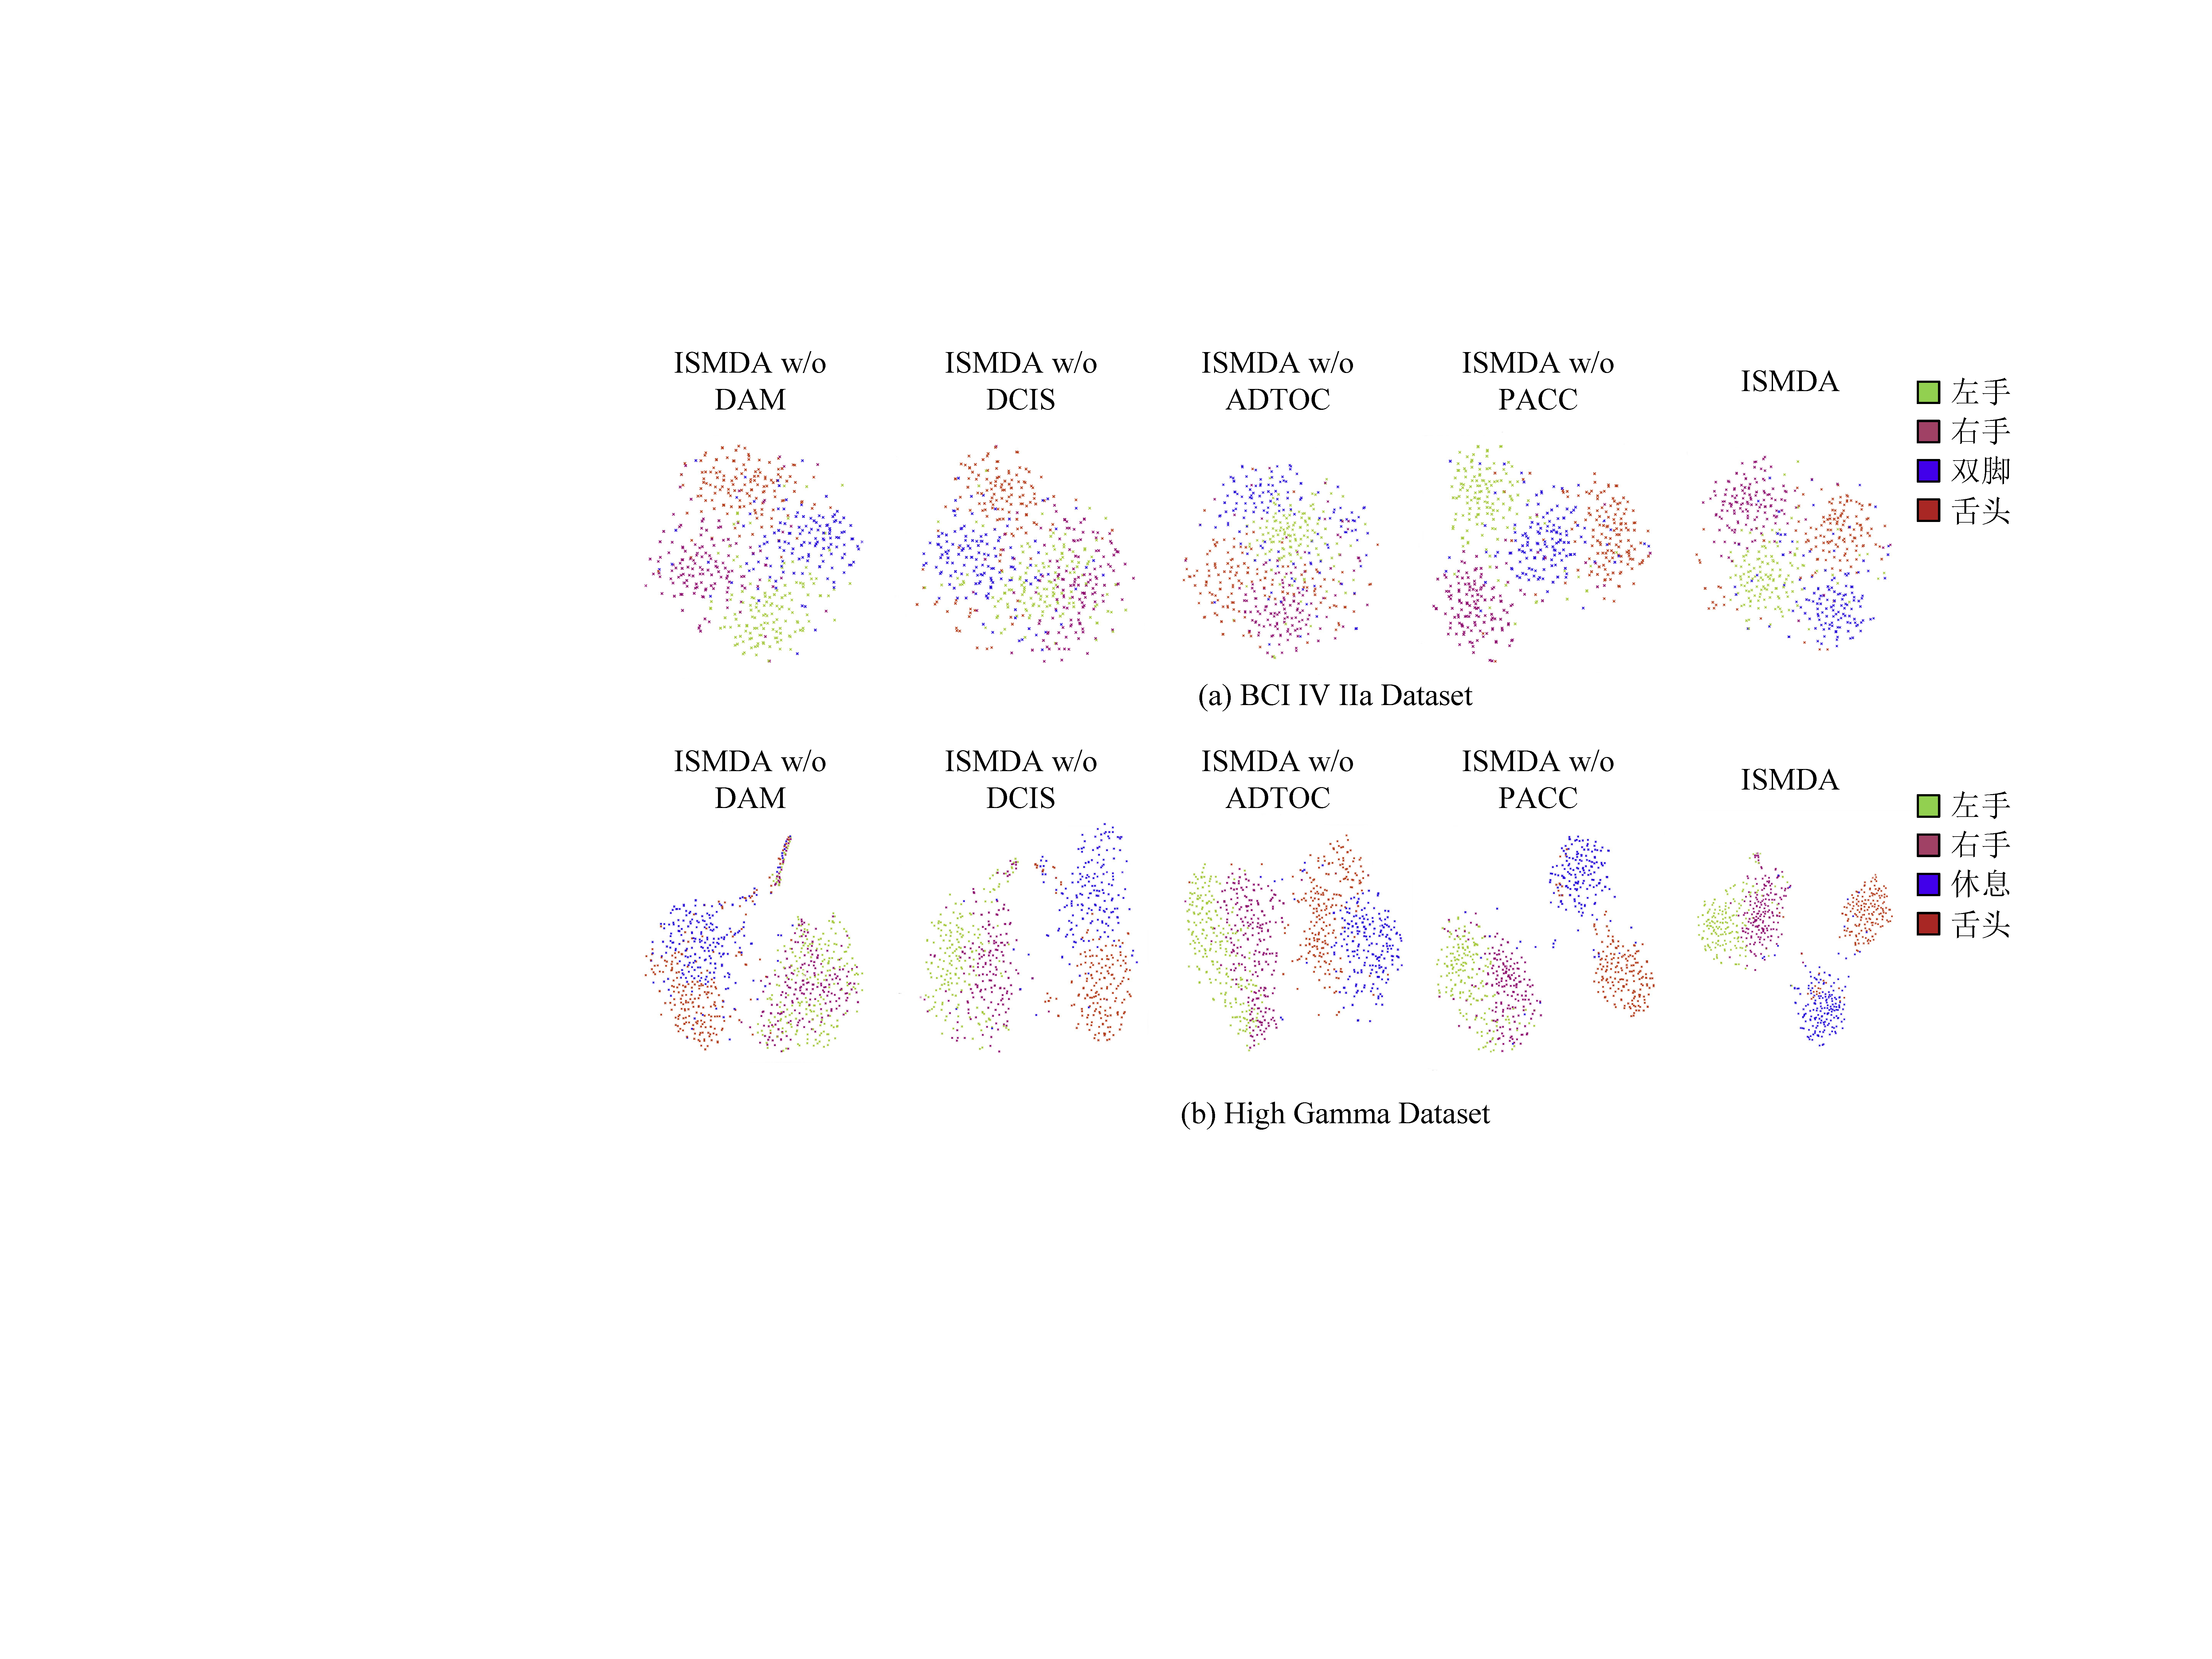
\includegraphics[width=0.9\textwidth]{特征图.pdf}
\caption{不同模型特征分布基于T-SNE可视化的结果}
\label{fig_4_6}
\end{figure*}

同样可以观察到,在High Gamma Dataset数据集上DAM的作用变得更加重要,这很可能是由于High Gamma Dataset更为庞大的源域数据量提供了更多的可以进行动态迁移的样本。这一推论可以在图\ref{fig_4_7}中得到证明,图\ref{fig_4_7}中在特征聚落之外出现了一些 “游离样本”(DAAN的右下角,CDAN的左侧,以及ISMDA w/o DAM的顶部)。这些独立的小集合包含了来自多个类别的样本,这无疑降低了模型的整体辨识精度。然而在图\ref{fig_4_6}的ISMDA w/o DCIS、ISMDA w/o ATDOC和ISMDA w/o PACC中,几乎所有这些“游离样本”都回到了各自相应的类别集群中。这意味着在一部分受试者的数据里,存在着无法通过“邻域聚合”或者“模型校准”完成正确分类的特殊样本。但是,这些特殊样本的分类可以通过学习具有相似特征的源域样本来完成。从另一个角度看,这也是本文引入迭代自训练机制的原因之一——在自训练时依然保持源域的知识有助于应对ADTOC无法解决的问题。
\begin{figure}[!h]
\centering
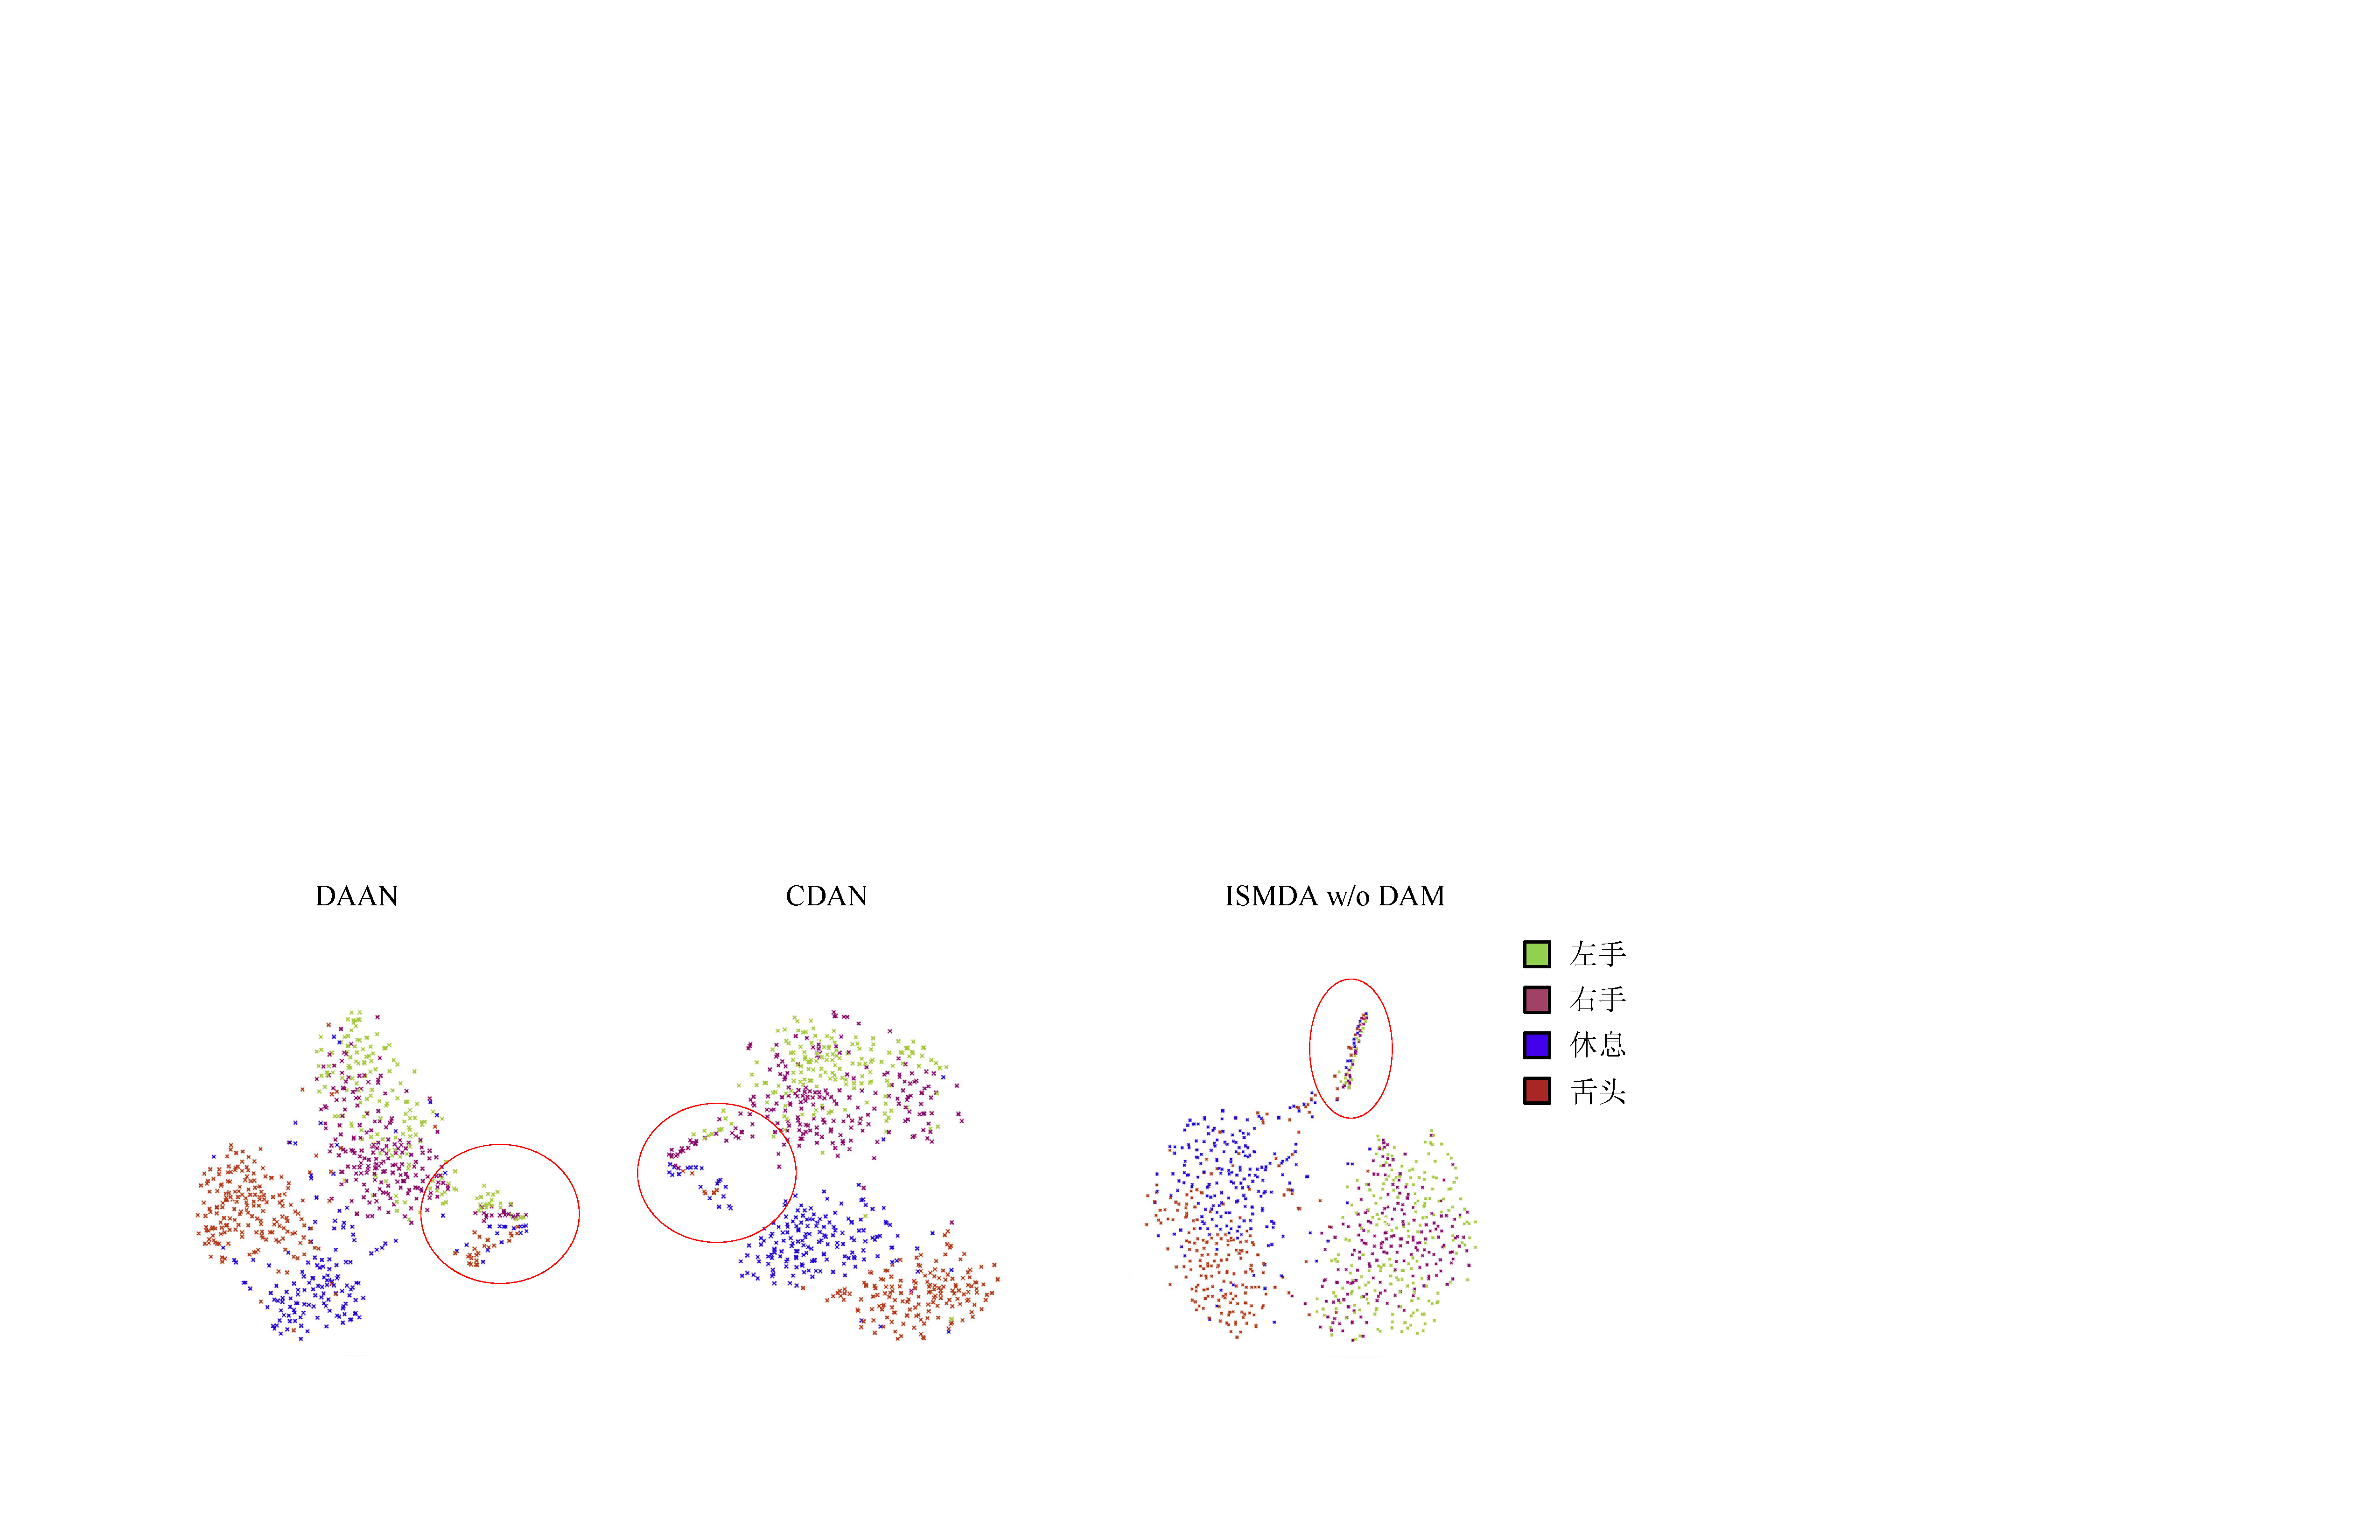
\includegraphics[width=0.99\textwidth]{离群点.pdf}
\caption{High Gamma Dataset中第五名被试的特征分布图}
\label{fig_4_7}
\end{figure}

(4) 超参数选取

DAM中的子空间路由由$K$个静态矩阵组成,这个超参数的选择影响了DAM的最终性能。本节对不同$K$的取值进行了消融实验,结果显示在表\ref{tab4-6}中。尽管参数变化带来的影响并不明显,但当$K$等于4时,模型的最终性能达到了最佳值。值得注意的是,由于Additional Dataset包含了数量庞大的被试,在所有被试身上进行消融实验时间成本较高,因此对于Additional Dataset的消融实验只在随机选择的一组受试者身上进行。即便如此,ISMDA在Additional Dataset上的最终结果仍然具有竞争力。毫无疑问,如果使用全部受试者进行超参数微调,ISMDA会获得更好的性能。选定受试者序号为1、47、46、37、13、27、12、32、53、54。


\begin{table*}[!h]
\caption{DAM中静态矩阵数$K$对于分类精度(\%)的影响\label{tab4-6}}
\centering
\wuhao{
    \begin{threeparttable}
    \setlength{\tabcolsep}{6mm}{
    \begin{tabular}{cccccc}
        \toprule
        \multirow{1}*{数据集}                & $K$=2   & $K$=4    & $K$=5   & $K$=8   & $K$=10 \\              
        \midrule
        BCI IV IIa  Dataset                 & 67.93 & 	\textbf{69.51} & 67.44 & 67.47 & 66.95 \\
        High Gamma Dataset                  & 81.61 & 	\textbf{82.38} & 81.34 & 80.92 & 79.85 \\
        Additional Dataset$^\dag$           & 89.80 & 	\textbf{91.30} & 90.60 & 90.50 & 88.60 \\
        JS-MI Dataset                       & 68.30 & 	\textbf{70.08} & 68.15 & 67.92 & 66.52  \\
        \bottomrule
    \end{tabular}
    }
    \begin{tablenotes}
            \footnotesize
	        \item {$\dag$}:实验仅在部分被试上进行。
            \item 高亮的结果:每一行中的最大值。
    \end{tablenotes}
\end{threeparttable}
}
\end{table*}


\subsection{面向域分类器的迭代自训练策略的有效性}
本节同样从分类精度、域间差异、特征分布以及超参数四个角度探索DCIS模块所带来的影响。

(1) 分类精度

与DAM不同,DCIS的引入进一步加强了模型对目标域数据的关注,给表\ref{tab4-5}中的ISMDA w/o DAM带来了两个显著变化。首先,由于ATDOC只面向目标域数据,它不会受到大量偏向右手类别的源域数据的影响。因此,尽管仍有轻微的偏向于右手,模型对右手和左手类别的辨别已经变得更加平衡。同样的现象也发生在舌头和休息之间。其次,DAM和DCIS在四个数据集上表现出了不同的重要性。在样本数相对较少的BCI IV IIa Dataset与JS-MI Dataset上,DCIS因为能够拉大不同类别的样本间距离而具有更好的效果。在数据量较多的High Gamma Dataset与Additional Dataset上,DAM因为可以从源域迁移更多种类的样本而带来了更大的性能提升。

为了反应ATDOC和PACC在DCIS中的重要性,本节对其分别进行了消融实验。从表\ref{tab4-5}中的ISMDA、ISMDA w/o ATDOC和ISMDA w/o PACC之间的比较来看,ATDOC是为模型带来更大性能提升的算法。当ATDOC被弃用时,模型在BCI IV IIa Dataset上的性能出现了明显下降。产生这一现象的主要原因是:尽管PACC可以校准模型,但它不能消除源域和目标域分布之间的域偏差的影响。

然而,加入PACC在一定程度上提高了模型分类的准确性,尤其是提高了模型对于休息类别的分类精度。同时,它稍微缓解了左手和右手之间的混淆程度。这一现象验证了PACC的设计初衷,即减少伪标签噪声带来的影响,去除高置信度的错误分类样本以及校准模型。

(2) 域间差异

在图\ref{fig_4_5}中,去除DCIS对BCI IV IIa Dataset和JS-MI Dataset带来了更大的影响。而在High Gamma Dataset和Additional Dataset上,DAM更为重要。这一结果展示了DAM和DCIS模块在四个数据集上关于域间差异的不同优势。在图\ref{fig_4_5}中的ATDOC和PACC之间,ATDOC仍然起着更重要的作用。这一结果表明,在训练的第一阶段,考虑目标域中特征之间的相似性是至关重要的。没有经过第一阶段的模型,即使经过模型校正,也很难达到预期的性能。尽管采用PACC并没有带来明显的变化,但在四个不同的数据集中,它均在一定程度上改善了模型性能,这反映了这种方法的泛化能力。

(3) 特征分布

从图\ref{fig_4_6}中可知,左手和右手类别的聚类往往倾向于相邻甚至会出现部分混合。同时,这一现象在图\ref{fig_4_7}的DAAN和CDAN之中也十分明显(DAAN和CDAN采用了与ISMDA相同的特征提取器MTSF)。这验证了前文对于表\ref{tab4-5}的结论——用卷积核大小为18的时间滤波器同时对左手和右手的频域特征进行提取,导致了难以对二者进行有效区分。在休息/脚和舌头之间也有明显的样本混淆,但情况并没有左手和右手之间那么棘手。这可能来源于尽管休息/脚的频率特征与舌头类似,但休息/脚有一套单独的卷积核大小为36的低频时间滤波器。由于这个原因,这两类样本可以更有效地区分开来。

ATDOC和PACC带来的变化可以更直观地在特征分布中看出,特别是在High Gamma Dataset中。ATDOC增加了不同类别之间的距离,明显地将四个类别分为两部分,并减少了类别间重叠。PACC则进一步增强了左手和右手样本之间的分离趋势,提升了模型性能。

(4) 超参数带来的影响

DCIS在Additional Dataset上的消融实验采用了与DAM相同的被试组合。本节对DCIS的两个模块——ATDOC和PACC的超参数分别进行分析。对于ATDOC,其性能依赖于最近邻样本数$m$。如表\ref{tab4-7},随着$m$变化,模型性能也不断发生改变,在$m=5$时模型性能达到最优值。BCI IV IIa Dataset和JS-MI Dataset对于$m$的变化更为敏感,这主要是由于ATDOC在这两个数据集上扮演着更为重要的角色。同时,在$m$的某些极端值下,ATDOC甚至对整个模型产生了一定的负面影响,使模型的分类性能比仅有DAM时更差。当$m$较小时,ATDOC的判断很容易受到个别极端特征点的影响;而当$m$较大时,混合不同类别的近邻集合会混淆分类器的判断,使模型性能下降。相反,High Gamma Dataset和Additional Dataset因为有着更多可迁移的源域样本,因此其对$m$的变化耐受度更高。

\begin{table*}[!h]
\caption{ATDOC中最近邻样本数$m$对于分类精度(\%)的影响\label{tab4-7}}
\centering
\wuhao{
    \begin{threeparttable}
    \setlength{\tabcolsep}{2.6mm}{
    \begin{tabular}{ccccccccc}
        \toprule
        \multirow{1}*{数据集}  & $m$=2   & $m$=3    & $m$=4   & $m$=5   & $m$=6  & $m$=7     & $m$=8    & $m$=9     \\        
        \midrule
        BCI IV IIa  Dataset                 & 64.25 & 	66.71 & 66.35 & \textbf{69.51} & 67.23 & 67.93     & 66.07     &  64.62    \\
        High Gamma Dataset                         & 78.54 & 	81.58 & 81.61 & \textbf{82.38} & 81.03 & 81.27     & 78.52     &  79.01    \\
        Additional Dataset$^\dag$   & 89.60 & 	90.60 & 90.10 & \textbf{91.30} & 89.80 & 90.20     & 89.10     &  88.70    \\
        JS-MI Dataset               & 65.40 &68.29 &66.95 &\textbf{70.08} & 68.02 & 68.55     & 67.25     &  64.93    \\  
        \bottomrule
    \end{tabular}
    }
    \begin{tablenotes}
            \footnotesize
	        \item {$\dag$}:实验仅在部分被试上进行。
            \item 高亮的结果:每一行中的最大值。
    \end{tablenotes}
\end{threeparttable}
}
\end{table*}

对于PACC,先前的研究指出\cite{4-9,4-27},没有必要对伪标签算法中的超参数,特别是“阈值”一类的超参数进行过度调节(over-tweak),因为它们本质上是较为鲁棒的。因此,尽管PACC中的超参数是在BCI IV IIa Dataset进行调整得到的,它们仍然在不同的数据集上取得了成功的结果。PACC中三个超参数的选择遵循以下过程:首先,选择置信度阈值$k_c$,只保留高置信度的伪标签。其次,基于置信度阈值,模型的Dropout概率被连续调整$U$次。最后,在前两者的基础上引入不确定性阈值$k_u$。这些结果是在之前选择的参数保持在最佳值时得到的。

\begin{table*}[!h]
\caption{PACC中超参数在BCI IV IIa Dataset上的影响\label{tab4-8}}
\centering
\wuhao{
    \begin{threeparttable}
    \setlength{\tabcolsep}{2.1mm}{
    \begin{tabular}{cccccccc}
        \toprule
        \multirow{1}*{超参数}                      &\multicolumn{7}{c}{超参数取值以及对应的准确率(\%)}\\ 
        \midrule
        \multirow{2}*{置信度阈值$k_c$}       & $k_c$=0.3 & $k_c$=0.4  & $k_c$=0.5 & $k_c$=0.6 & $k_c$=0.7 & $k_c$=0.8 & $k_c$=0.9\\     
                                                        & 66.75   & 66.82    & 67.29   & 67.46   & \textbf{67.85}   &  67.49  & 67.31  \\
        % \midrule
        \multirow{2}*{Dropout调整次数$U$}                & $U$=5     & $U$=10     & $U$=20    & $U$=30    & $U$=40    & $U$=50    & $U$=60\\   
                                                        & 67.92   & 68.17    & 68.31   & 68.65   & 68.67   & 68.72   & \textbf{68.73}\\
        % \midrule
        \multirow{2}*{不确定性阈值$k_u$}                 &$k_u$=0.01 &$k_u$=0.03  &$k_u$=0.05 &$k_u$=0.08 &$k_u$=0.10 &$k_u$=0.15 &$k_u$=0.20\\
        
                                                        & 68.79   & 69.32    & \textbf{69.51}   & 69.29   & 68.93   & 68.54   & 68.05\\
        \bottomrule
    \end{tabular}
    }
    \begin{tablenotes}
            \footnotesize
	        \item {$\dag$}:实验仅在部分被试上进行。
            \item 高亮的结果:每一行中的最大值。
    \end{tablenotes}
\end{threeparttable}
}
\end{table*}

如表\ref{tab4-8}所示,当$k_c$小于0.5时,大量的低置信度样本使模型的性能甚至低于ISMDA w/o PACC。当$k_c$超过0.5时,会使模型具有相对稳定的性能。然而,当阈值太高时,将只有少数的样本可以通过筛选,这限制了模型的最终发展。与其他超参数不同,PACC中$U$的影响并不明显。毫无疑问,随着$U$的增加,模型的最终准确率将逐渐上升,因为它消除了随机性带来的干扰。然而,可以看到,当$U$超过30时,模型性能的提高趋近于饱和。综合考虑模型性能和计算资源的消耗,选取$U$的值为30。$k_u$的选择与$k_c$类似。当$k_u$大于0.1时,太多高不确定性的伪标签进入模型,导致精度下降。然而,当$k_u$较小时,也会出现性能下降,因为只有少量的伪标签能通过筛选。

\subsection{损失函数中分量权重带来的影响}
对于总损失函数中三个分量的权重,本节按照与设计时相同的步骤进行相应的消融实验。首先,将不同权重的$\mathcal{L}_{d o c}^{t}$加入到$\mathcal{L}_{c l s}^{s}$中。其次,在第二阶段对$\mathcal{L}_{c l s}^{s}$进行了缩放,以对模型进行微调。这种缩放使模型能够保留源域的知识,并且不会产生过度拟合。最后,在第一阶段的最优模型上,引入不同权重的$\mathcal{L}_{c l s}^{t}$进行对比。

\begin{table*}[!h]
\caption{损失函数中不同分量权重的消融实验\label{tab4-9}}
\centering
\wuhao{
\begin{threeparttable}
\setlength{\tabcolsep}{1.8mm}{
    \begin{tabular}{cccccccc}
        \toprule
        \multicolumn{8}{c}{\textbf{$\mathcal{L}_{d o c}^{t}$权重$\beta_{0}$对准确率(\%)的影响}}\\    
        \midrule
        \multirow{1}*{数据集}                &$\beta_{0}$=0.01&$\beta_{0}$=0.02&$\beta_{0}$=0.05&$\beta_{0}$=0.1&$\beta_{0}$=0.2&$\beta_{0}=0.5$&  $\beta_{0}=1.0$\\              
        \midrule
        BCI IV IIa Dataset                           & 64.15 & 	64.17 & 65.43 & 66.05 & \textbf{67.27} & 66.54  & 65.86 \\
        High Gamma Dataset                                     & 80.96 & 	\textbf{81.33} & 80.71 & 80.04 & 80.01 & 78.35  & 77.06 \\
        Additional Dataset$^\dag$              & 90.00 & 	\textbf{90.20} & 89.80 & 88.60 & 88.70 & 87.60  & 86.30 \\
        JS-MI Dataset                          & 66.53 & 	67.28 & 68.31 & 68.92 & \textbf{69.20} & 68.14  & 67.42 \\
        \midrule
        \multicolumn{8}{c}{\textbf{$\mathcal{L}_{c l s}^{s}$的缩放系数对准确率(\%)的影响}}\\    
        \midrule
        \multirow{1}*{数据集}                & 0.01    & 0.02    & 0.05    & 0.1     & 0.2     & 0.5      & 1.0  \\        
        \midrule
        BCI IV IIa Dataset                            & 67.27 & 67.33 & 67.30 & \textbf{67.50} & 67.01 & 65.85  & 64.07 \\
        High Gamma Dataset                                     & 81.40 & 81.49 & 81.58 & \textbf{81.64} & 80.71 & 79.83  & 78.05 \\
        Additional Dataset$^\dag$              & 90.30 & 90.20 & 90.30 & \textbf{90.40} & 89.50 & 88.70  & 87.20 \\
        JS-MI Dataset                          & 69.29 & 69.28 & 69.55 & \textbf{69.85} & 68.74 & 68.15  & 67.64 \\
        \midrule
        \multicolumn{8}{c}{\textbf{$\mathcal{L}_{cls}^{t}$权重$\gamma_{0}$对准确率(\%)的影响}}\\      
        \midrule
        \multirow{1}*{数据集}                &$\gamma_{0}=0.1$&$\gamma_{0}=0.2$&$\gamma_{0}=0.5$&$\gamma_{0}=1.0$&$\gamma_{0}=2.0$&$\gamma_{0}=3.0$& $\gamma_{0}=4.0$ \\        
        \midrule
        BCI IV IIa Dataset                            & 67.82 & 	68.65 & 68.62 & 69.08 & \textbf{69.51} & 68.59     & 67.41 \\
        High Gamma Dataset                                     & 81.70 & 	81.68 & 81.96 & 82.12 & \textbf{82.38} & 81.54     & 81.22 \\
        Additional Dataset$^\dag$              & 90.40 & 	90.50 & 90.90 & \textbf{91.30} & \textbf{91.30} & 90.20     & 89.40 \\
        JS-MI Dataset                          & 69.88 & 	69.90 & 69.86 & 69.94 & \textbf{70.08} & 69.09     & 68.51 \\
        \bottomrule
       
    \end{tabular}
    }
    \begin{tablenotes}
            \footnotesize
	        \item {$\dag$}:实验仅在部分被试上进行。
            \item 高亮的结果:每一行中的最大值。
    \end{tablenotes}
\end{threeparttable}
}

\end{table*}

由于从源域中学习更多有用的域泛化特征是本章的最终目标,因此ATDOC应当扮演辅助的角色——在第一阶段,ATDOC的损失权重$\beta_{0}$小于源域的交叉熵损失权重。如表\ref{tab4-9}所示,随着$\beta_{0}$的逐渐增大,模型的性能也发生了明显下降。因为过度依赖根据特征间的余弦相似度得到的分类结果,将会让模型舍弃本应在源域上获得的分类能力。综上所述,在所有数据集上,$\beta_{0}$均小于1。由于ATDOC和DAM在不同数据集上的重要性不同,ATDOC的权重也不同。Additional Dataset在$\beta_{0}$上表现出与High Gamma Dataset相似的特性。这归因于它仅包含两个类别,即使只有部分被试被采用,每个类别仍具有更多的样本供DAM完成动态迁移。和前面的分析一致,DAM的显著效果迫使模型选取相对较低的$\beta_{0}$。


$\mathcal{L}_{c l s}^{s}$的缩放系数的作用是在第二阶段保持模型对于源域的认知,并且不产生过度拟合。正如表\ref{tab4-9}所示,当该值设置为0.1时,模型满足上述要求。如果该值过大,模型的性能就会因过拟合而下降。如果该值太小,源域可能会因为PACC的引入而被遗忘。因此在公式\ref{eq:12A}中,第二阶段的$\alpha_0$被乘以0.1。

$\gamma_{0}$的作用是为了在第二训练阶段完成对模型的校准。因此,它大于第二阶段的$\mathcal{L}_{c l s}^{s}$的权重。随着$\gamma_{0}$的增加,模型逐渐完成了校准过程。然而,当$\gamma_{0}$过大时,模型过于偏向目标域,忽略了第一阶段学到的域不变特征,导致性能明显下降。所提出的方法选择了在所有数据集上均表现较好的$\gamma_{0}$的值。










\section{本章小结}

本章提出了一种名为迭代自训练多被试域适应的无监督域适应算法,用来完成对运动想象EEG信号的辨识任务。具体来说,本章提出了多通道时空滤波模块,从运动想象EEG的时频域提取关键性特征。引入动态注意力模块,根据输入数据的特征动态调整网络参数,削弱不同源域之间界限,减少对域信息的依赖。此外,本章还引入了基于面向域分类器的迭代自训练策略。在第一个训练阶段,面向目标域的辅助分类器被用来获得目标域的伪标签。在训练的第二阶段,基于确定性和置信度的伪标签算法选择高质量的伪标签来校准模型。为了验证模型的性能,并同时验证JS-AINS-40系统的可靠性,分别引入三个公开的和一个JS-AINS-40采集的运动想象数据集。所有的结果均表明,所提出的方法可以在多被试迁移学习任务上达到当前的最佳结果。


